\section{Results and Analysis}
\subsection{Overview}

This section presents the experimental results for the four priority queue
implementations used by Dijkstra's algorithm: binary, pairing, Fibonacci, and
Brodal--Okasaki heaps. Each implementation was evaluated using the seven input
graphs described in Section~3.2 and both Dijkstra variants: eager
\code{decrease_key} and \code{lazy} duplicate-entry processing.

We first compare execution time, both between heap implementations and between
the two Dijkstra variants. We then examine hardware performance counters and
memory measurements to identify factors that may explain the observed runtime
differences. The results are discussed with respect to graph size, density,
and structure, including uniform random, grid, hub-skewed, and layered graphs.

\subsection{Runtime Results}
\subsubsection{Runtime Comparison Between Heap Implementations}

Table~\ref{tab:dijkstra_runtime} reports the mean execution time of each heap
implementation across the seven input graphs. The corresponding graph-specific
runtime plots are shown in Figure~\ref{fig:runtime-heap-comparison}.

% Auto-generated by src/bench/plot.py
\begin{table}[H]
  \centering
  \small
  \caption{Dijkstra Execution Time across Heaps and Input Datasets (Mean $\pm$ 99\% Confidence)}
  \label{tab:dijkstra_runtime}
  \begin{tabular}{llrrrr}
    \toprule
    \textbf{Dataset} & \textbf{Mode} & \textbf{binary} & \textbf{brodal-okasaki} & \textbf{fibonacci} & \textbf{pairing} \\
    \midrule
    smoke\_1k & Decrease-Key & 30.99 µs & 228.21 µs & 137.81 µs & 46.95 µs \\
    & Lazy & 36.97 µs & 184.16 µs & 176.34 µs & 58.05 µs \\
    \addlinespace
    uniform\_sparse & Decrease-Key & 718.96 µs & 3.46 ms & 2.01 ms & 925.24 µs \\
    & Lazy & 873.17 µs & 2.82 ms & 2.36 ms & 1.08 ms \\
    \addlinespace
    uniform\_medium & Decrease-Key & 2.13 ms & 16.24 ms & 4.86 ms & 3.10 ms \\
    & Lazy & 3.25 ms & 10.49 ms & 8.04 ms & 4.84 ms \\
    \addlinespace
    uniform\_dense & Decrease-Key & 1.69 ms & 16.11 ms & 3.08 ms & 2.43 ms \\
    & Lazy & 3.18 ms & 9.57 ms & 7.04 ms & 4.26 ms \\
    \addlinespace
    grid\_224 & Decrease-Key & 2.40 ms & 12.49 ms & 7.23 ms & 3.58 ms \\
    & Lazy & 2.75 ms & 10.13 ms & 8.99 ms & 4.14 ms \\
    \addlinespace
    hub\_skewed & Decrease-Key & 1.54 ms & 6.43 ms & 4.09 ms & 2.53 ms \\
    & Lazy & 1.72 ms & 5.59 ms & 4.52 ms & 2.80 ms \\
    \addlinespace
    layered\_frontier & Decrease-Key & 1.15 ms & 11.97 ms & 3.69 ms & 2.08 ms \\
    & Lazy & 2.34 ms & 8.10 ms & 6.74 ms & 3.39 ms \\
    \addlinespace
    \bottomrule
  \end{tabular}
\end{table}


\begin{figure}[H]
  \centering
  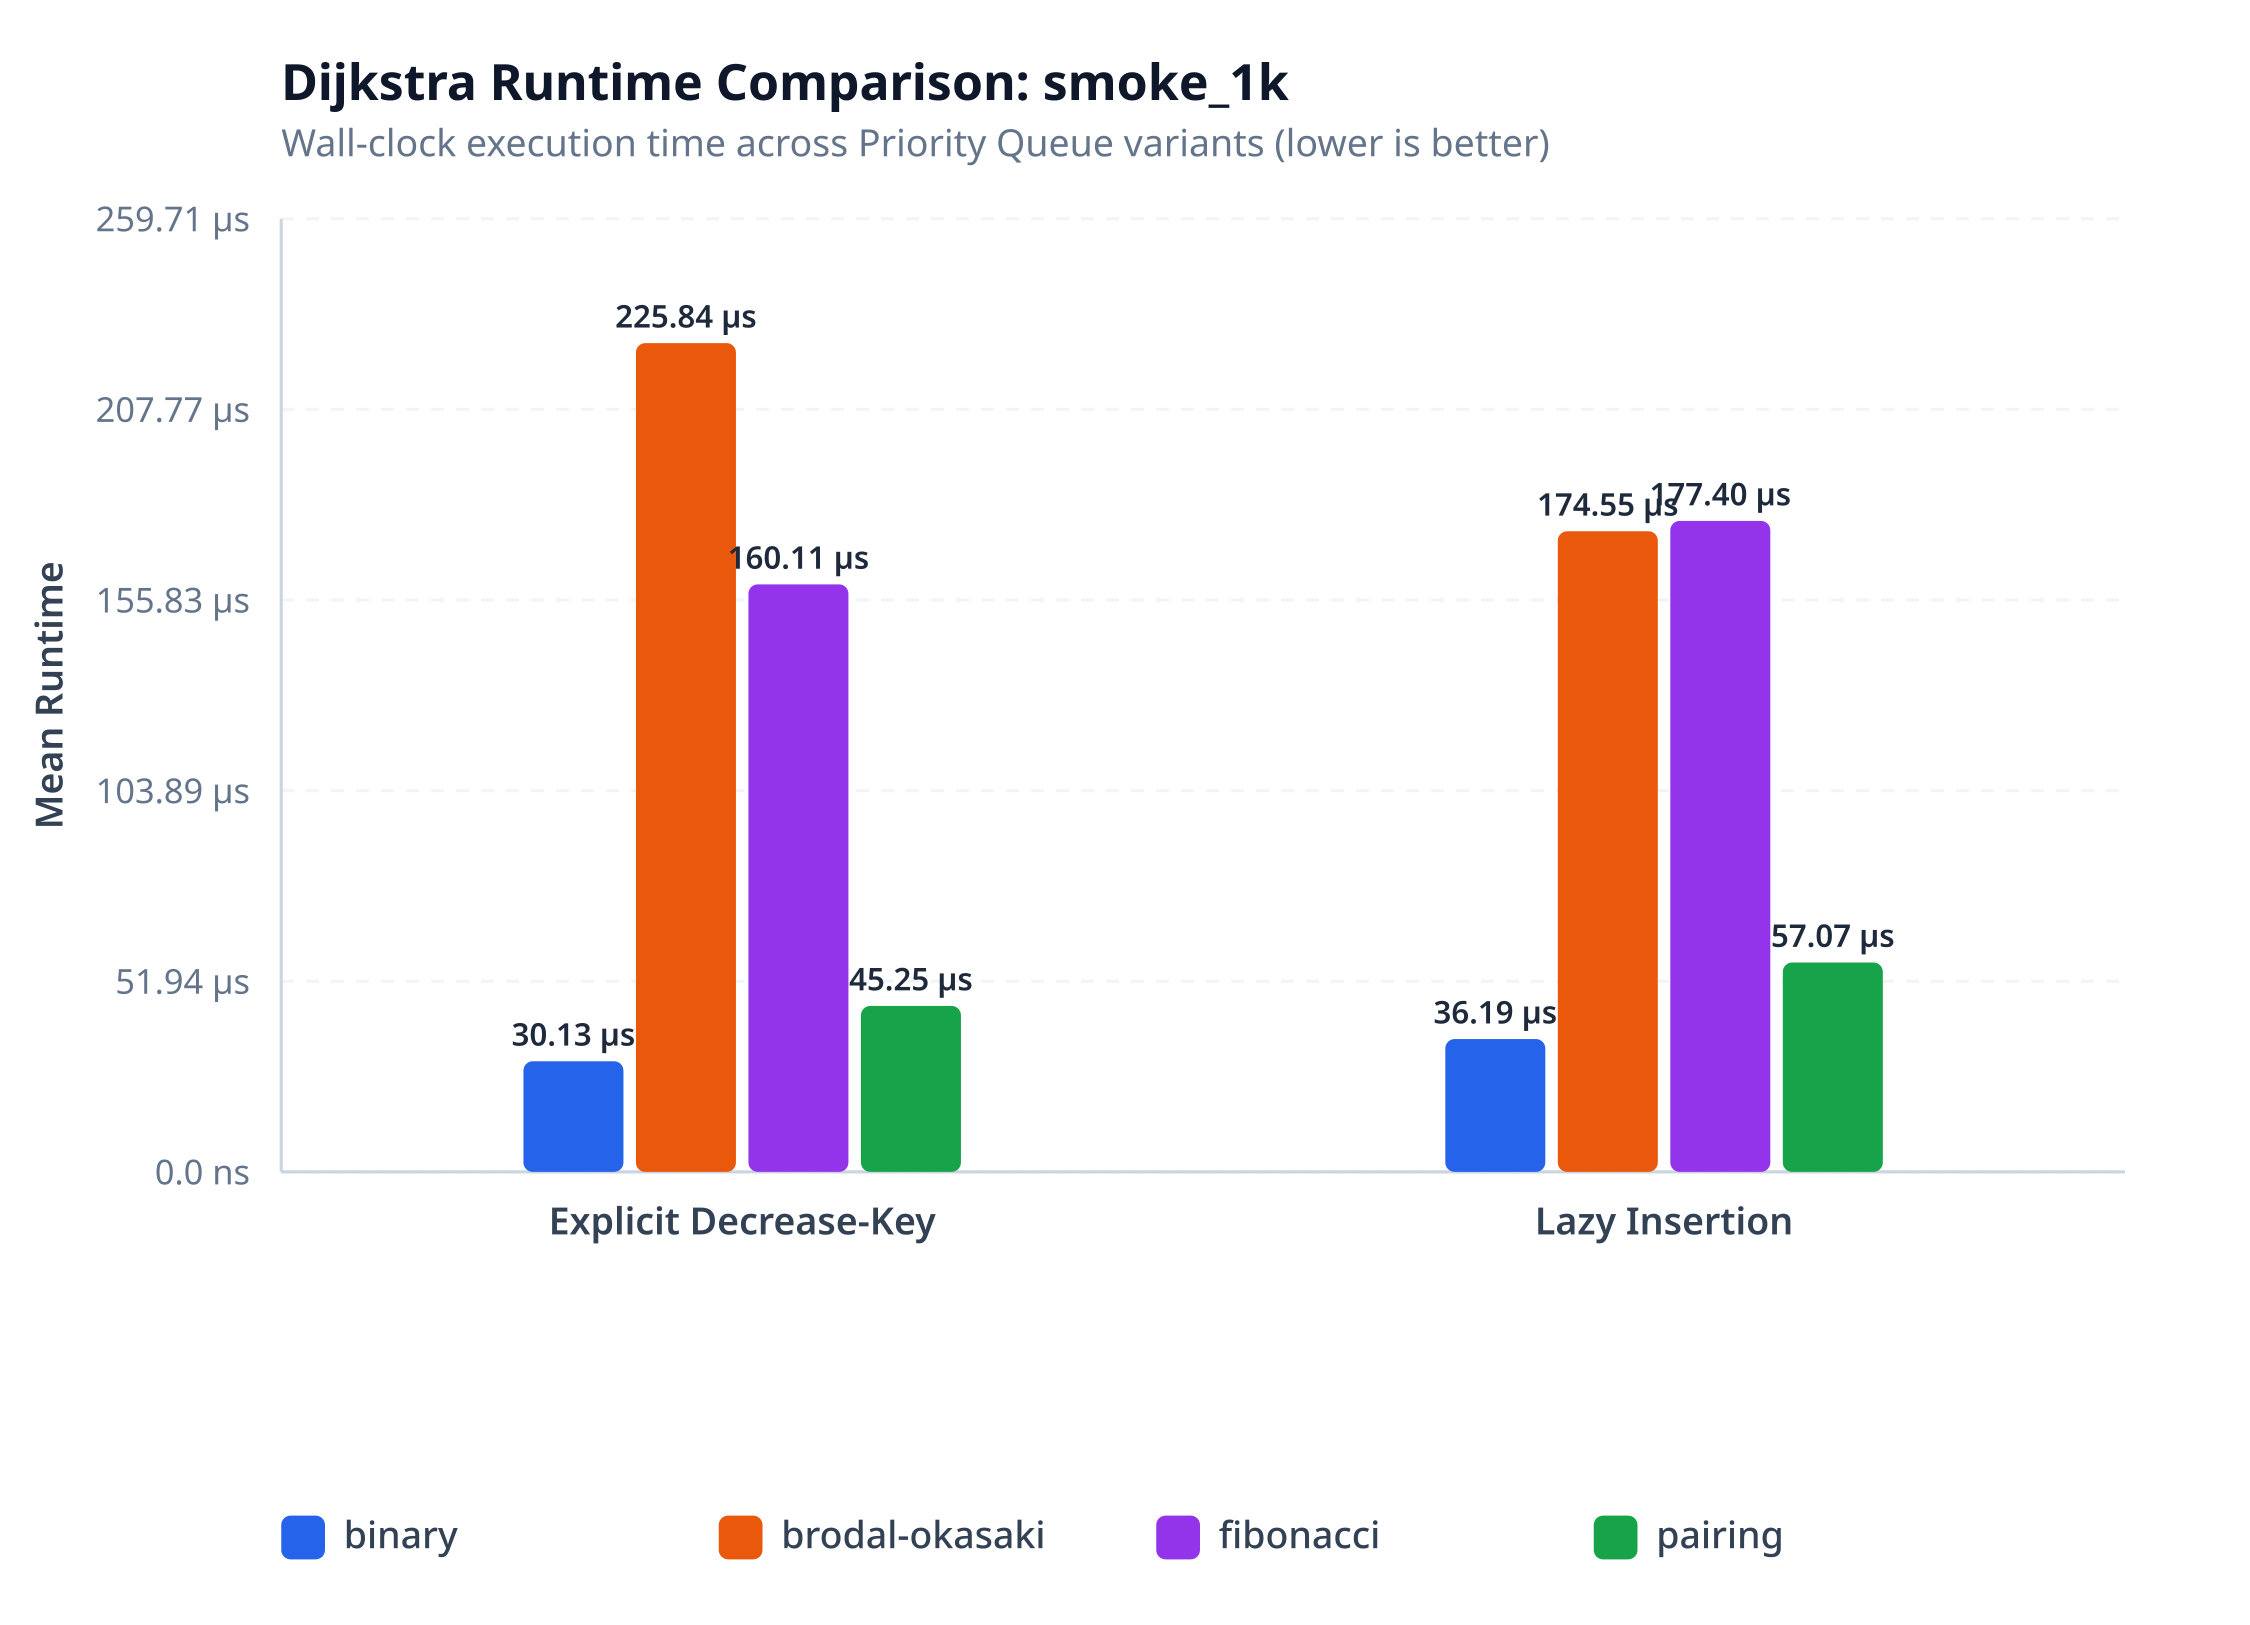
\includegraphics[width=0.48\textwidth]
    {frozen_results/figures/report_charts/runtime/smoke_1k.png}
  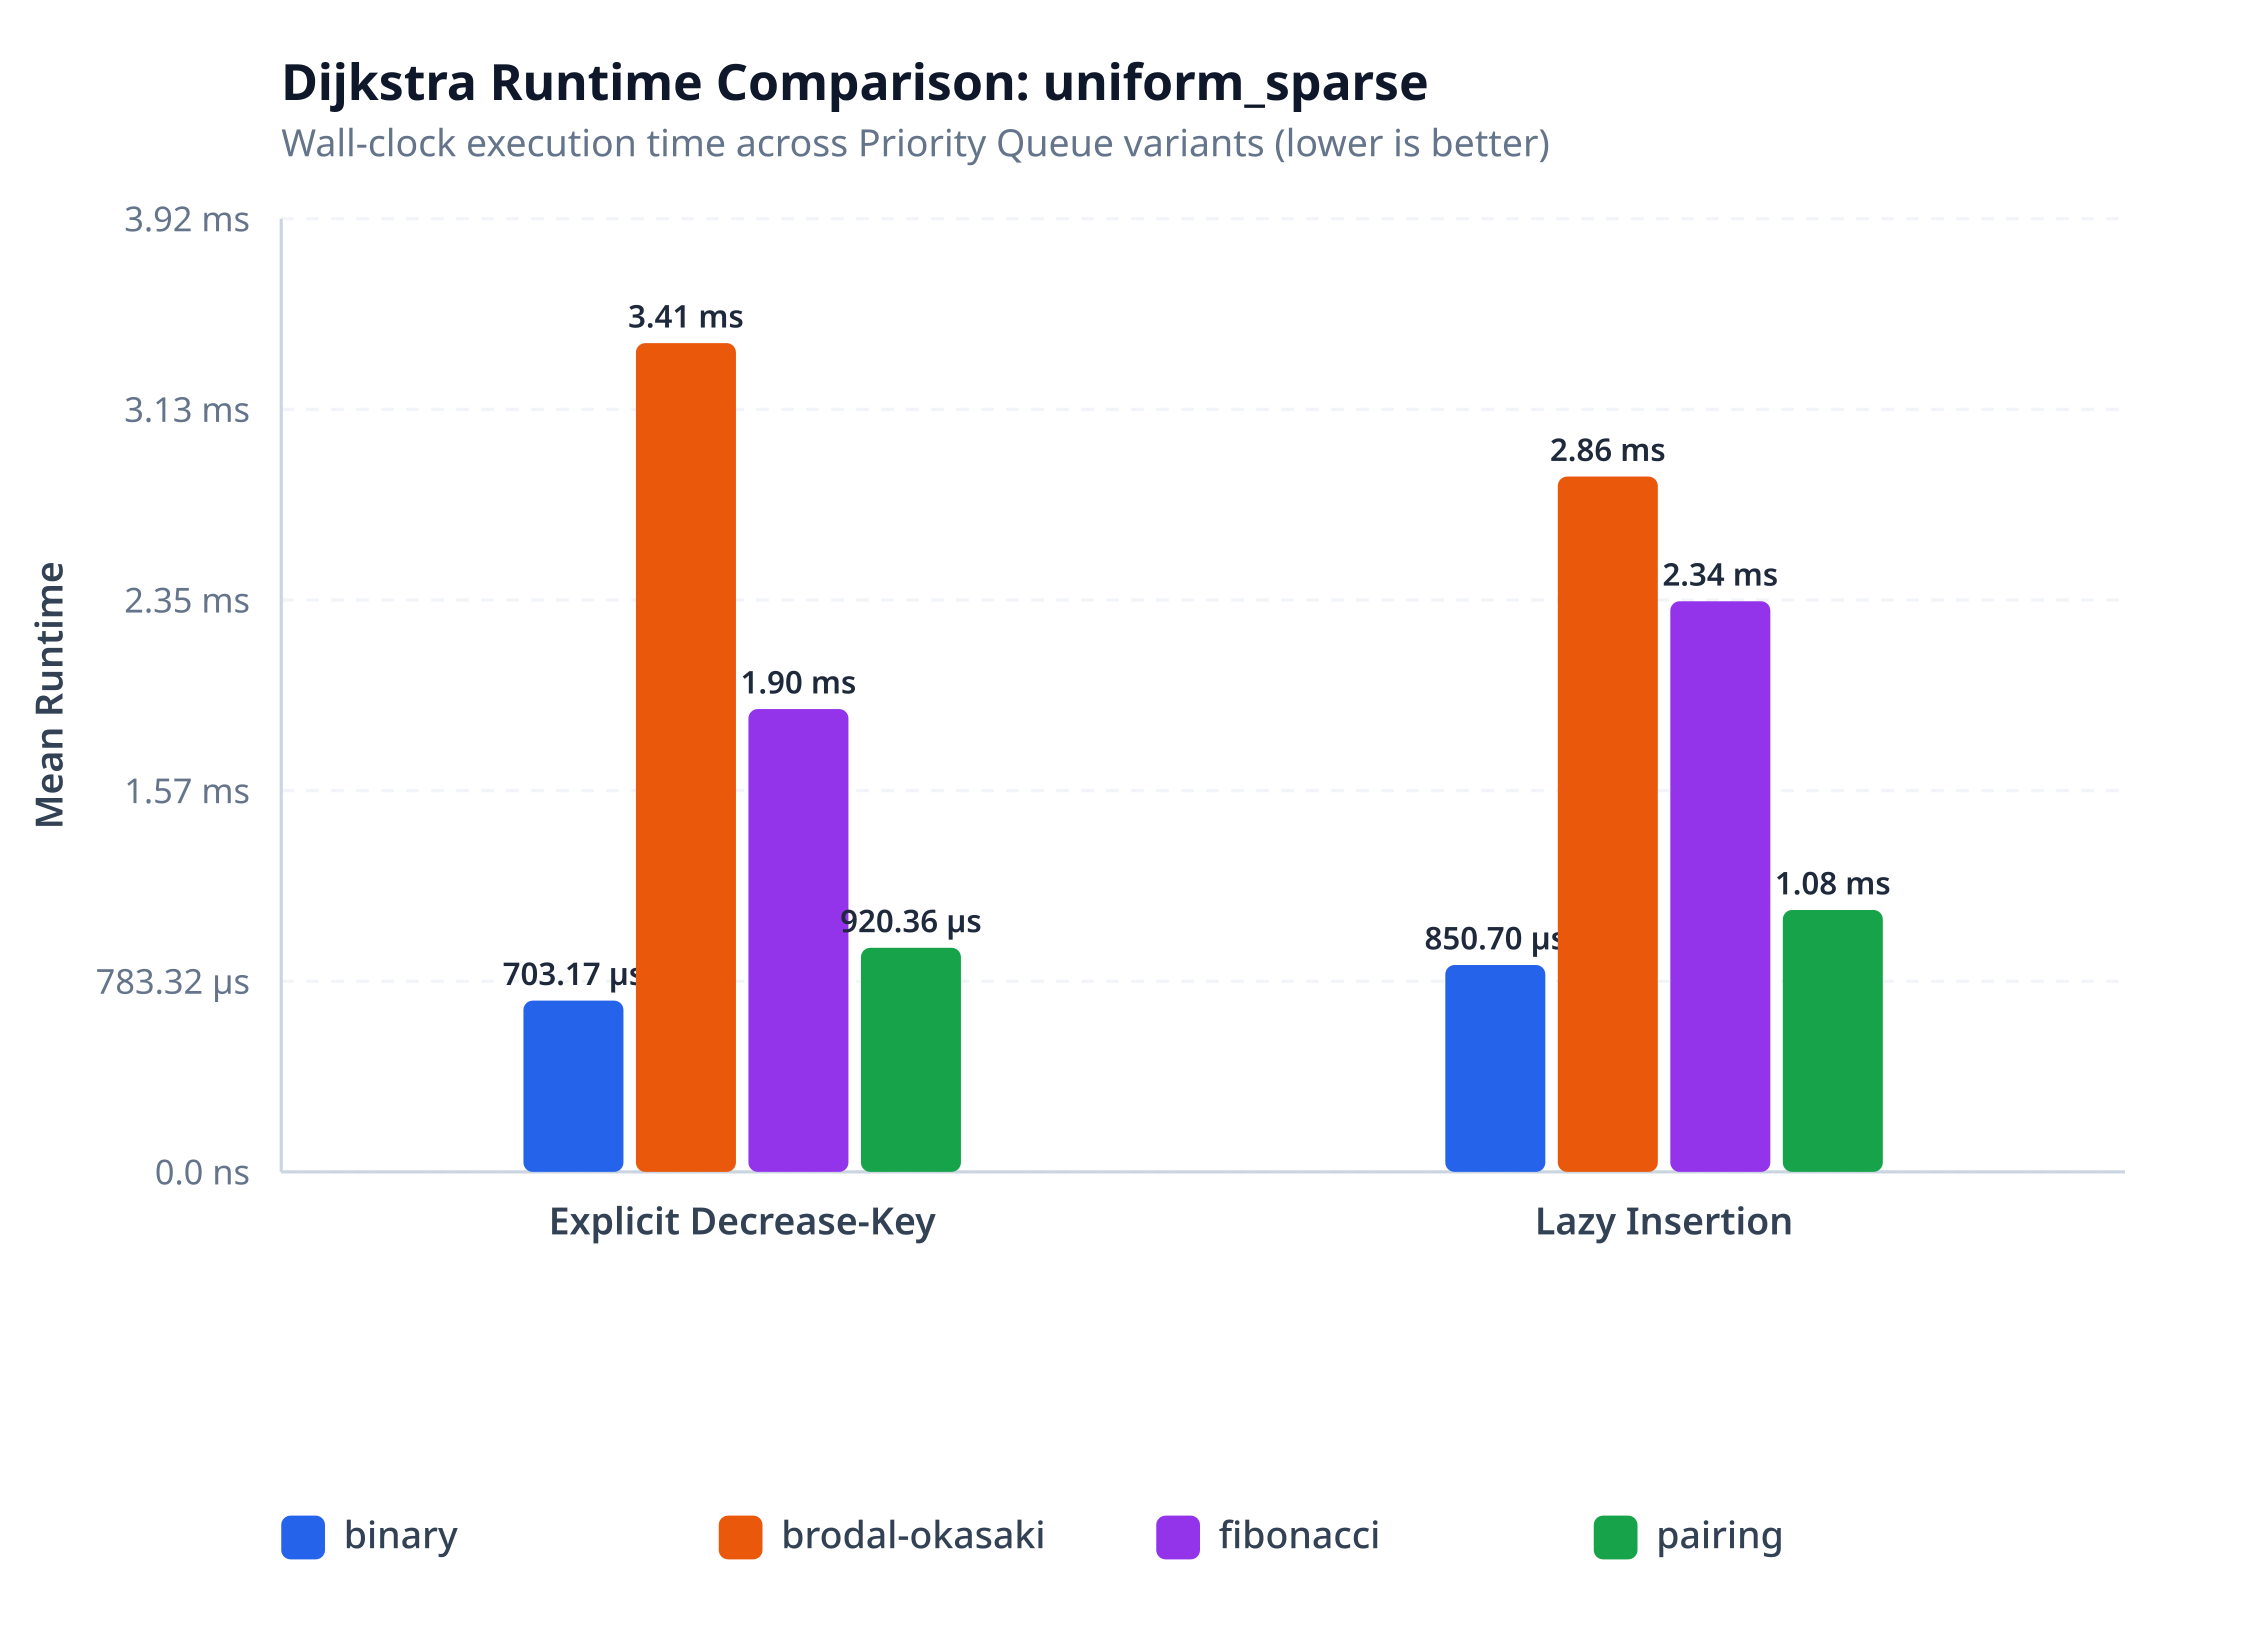
\includegraphics[width=0.48\textwidth]
    {frozen_results/figures/report_charts/runtime/uniform_sparse.png}

  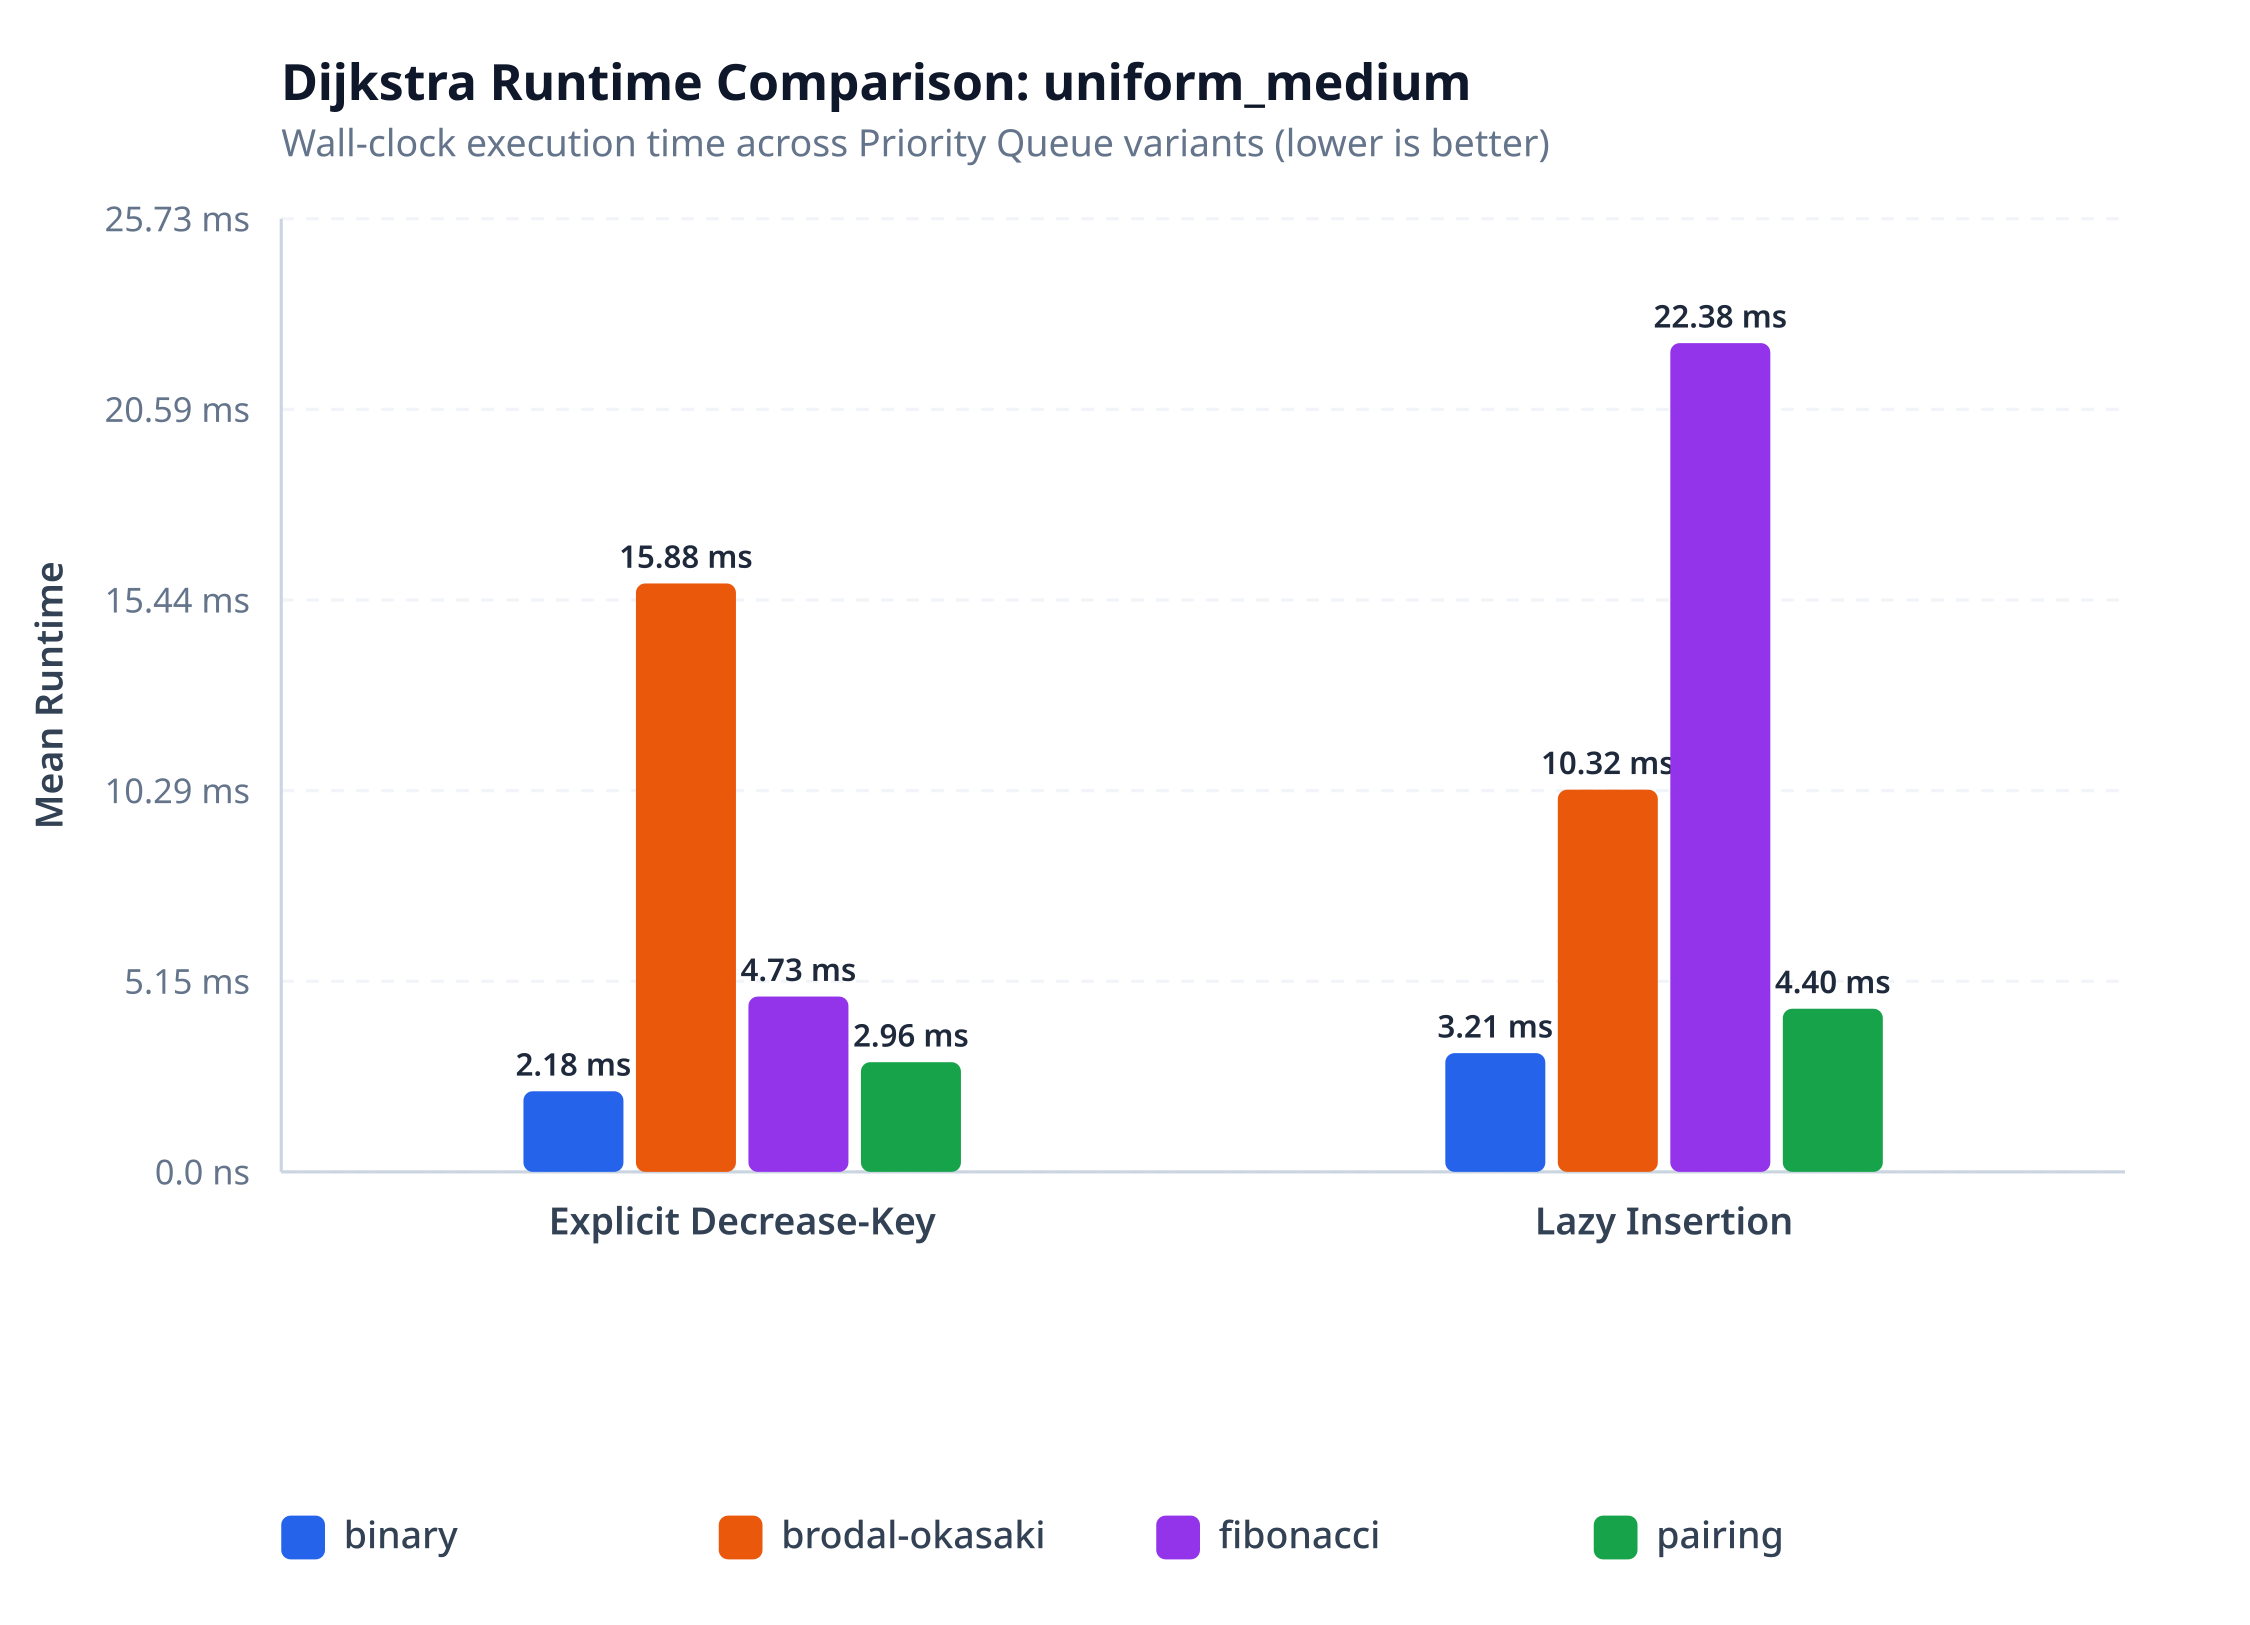
\includegraphics[width=0.48\textwidth]
    {frozen_results/figures/report_charts/runtime/uniform_medium.png}
  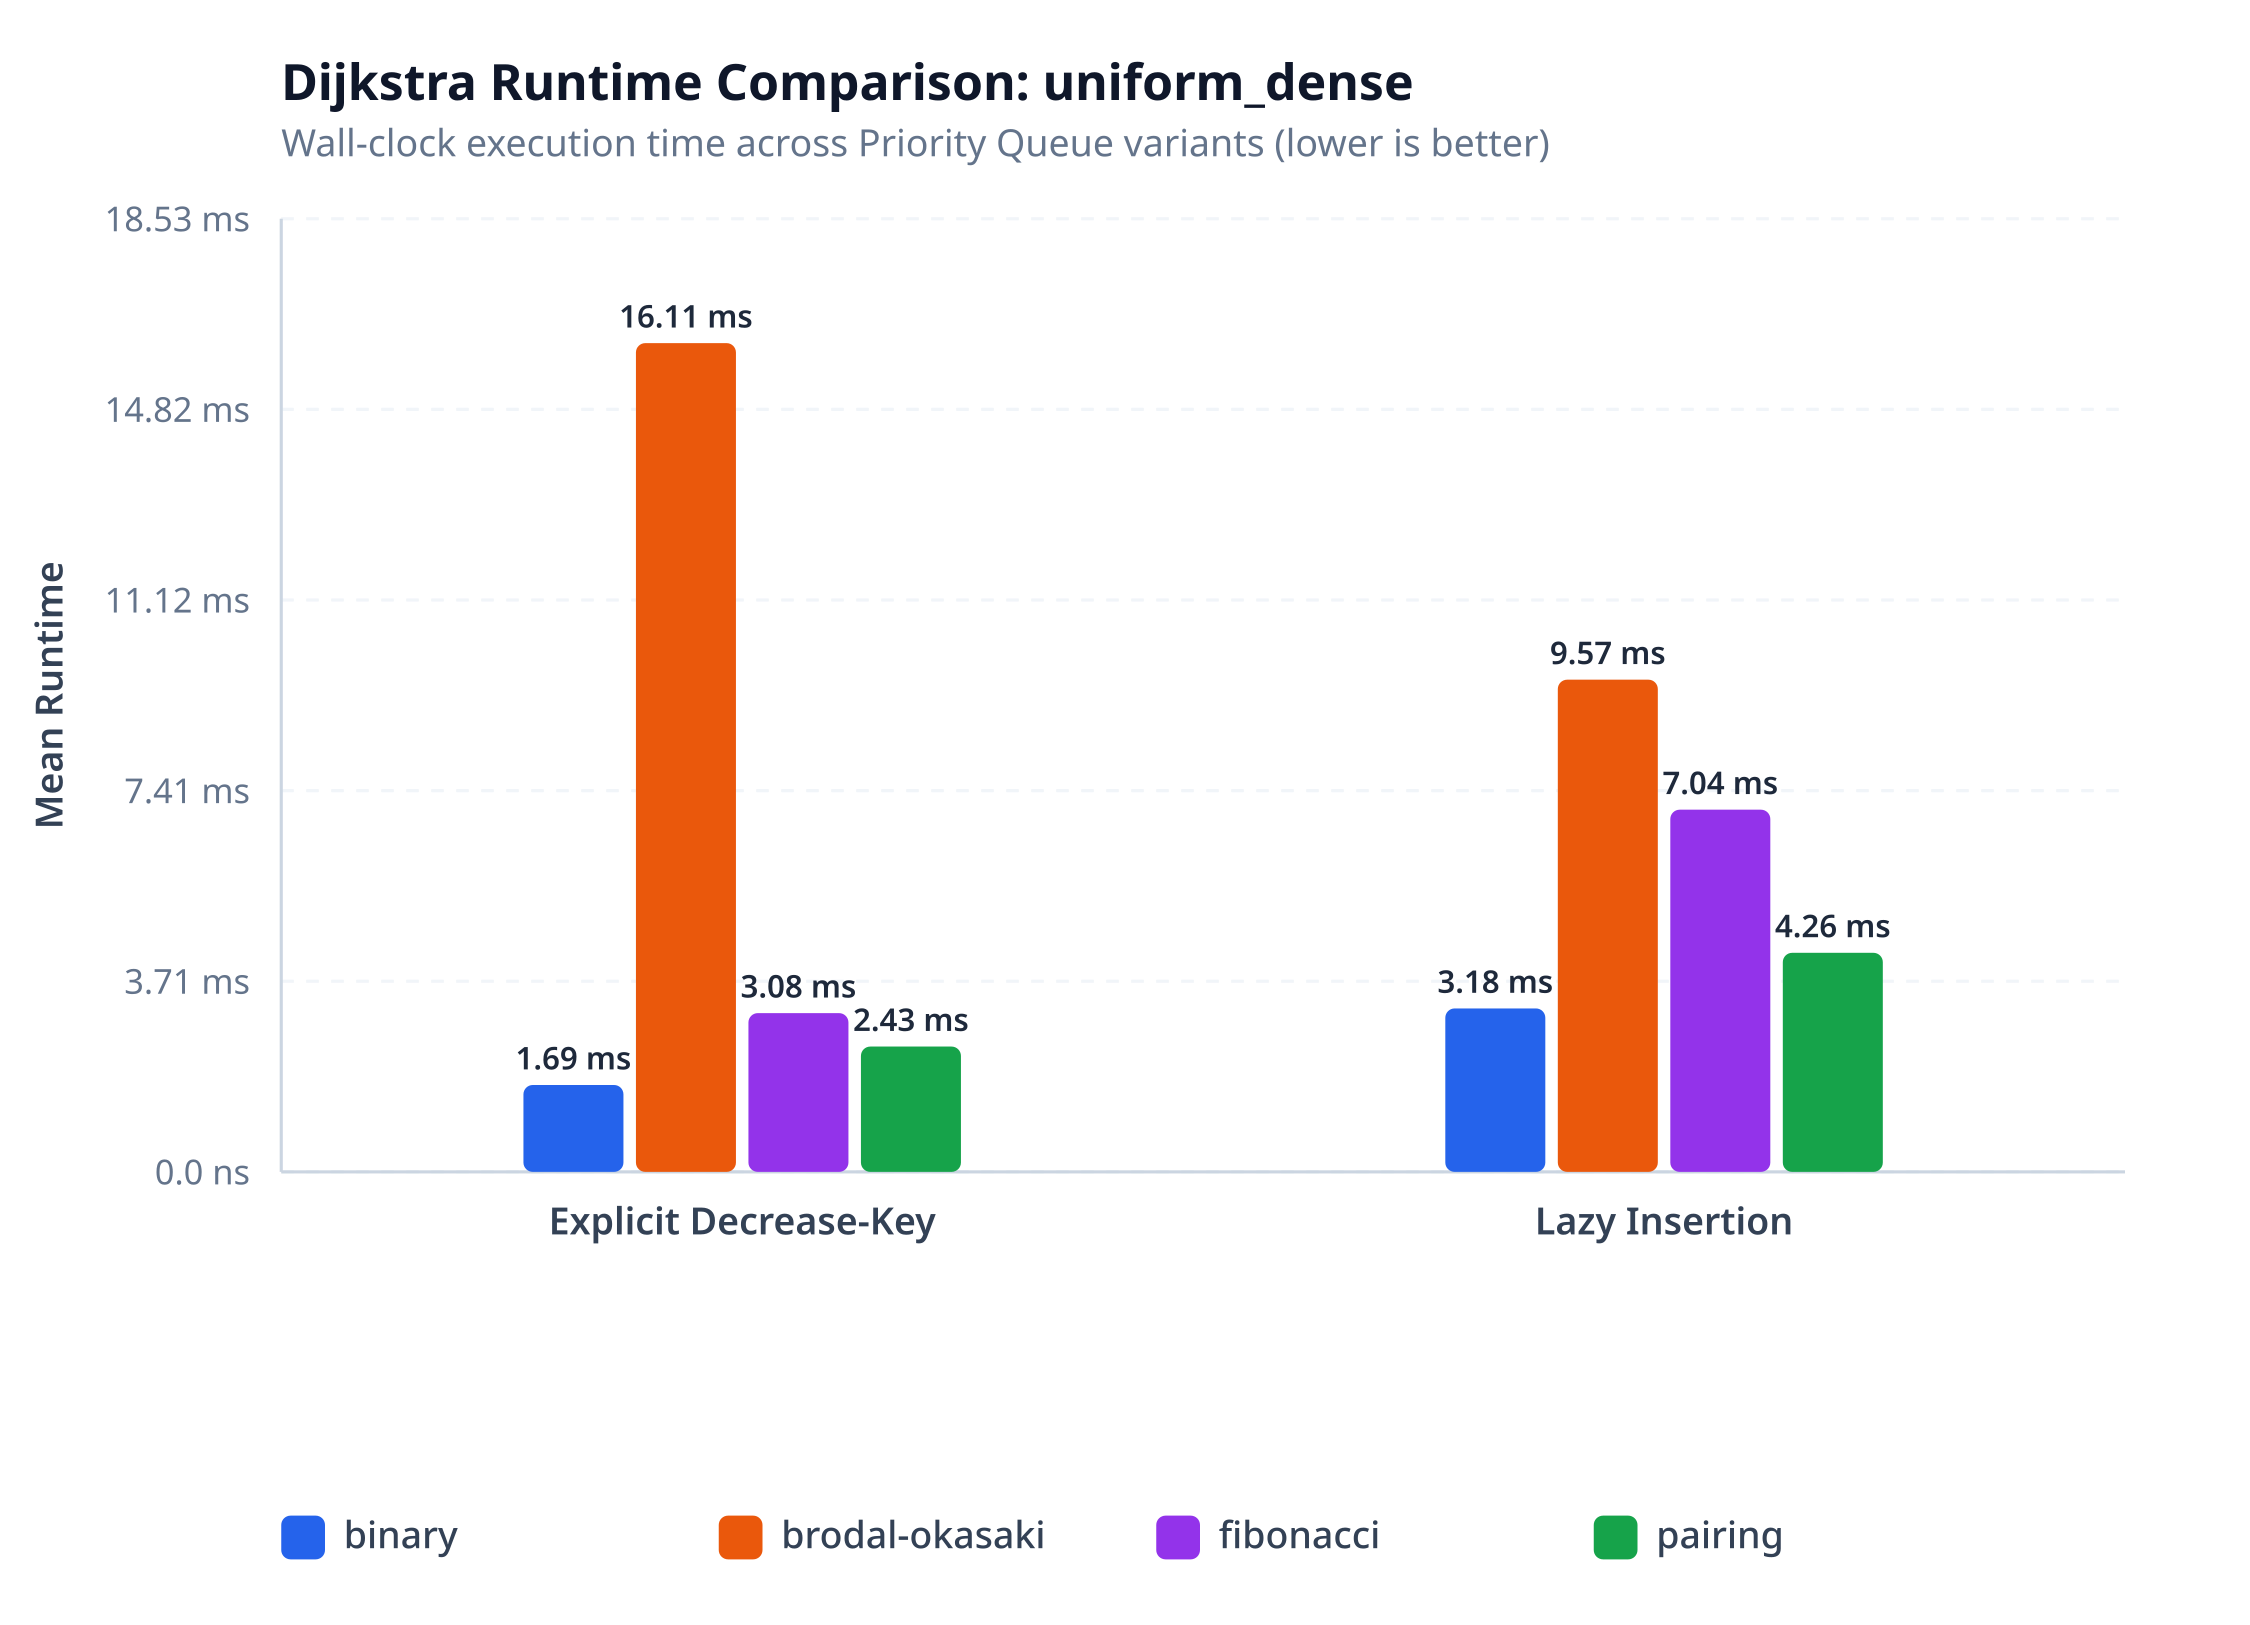
\includegraphics[width=0.48\textwidth]
    {frozen_results/figures/report_charts/runtime/uniform_dense.png}

  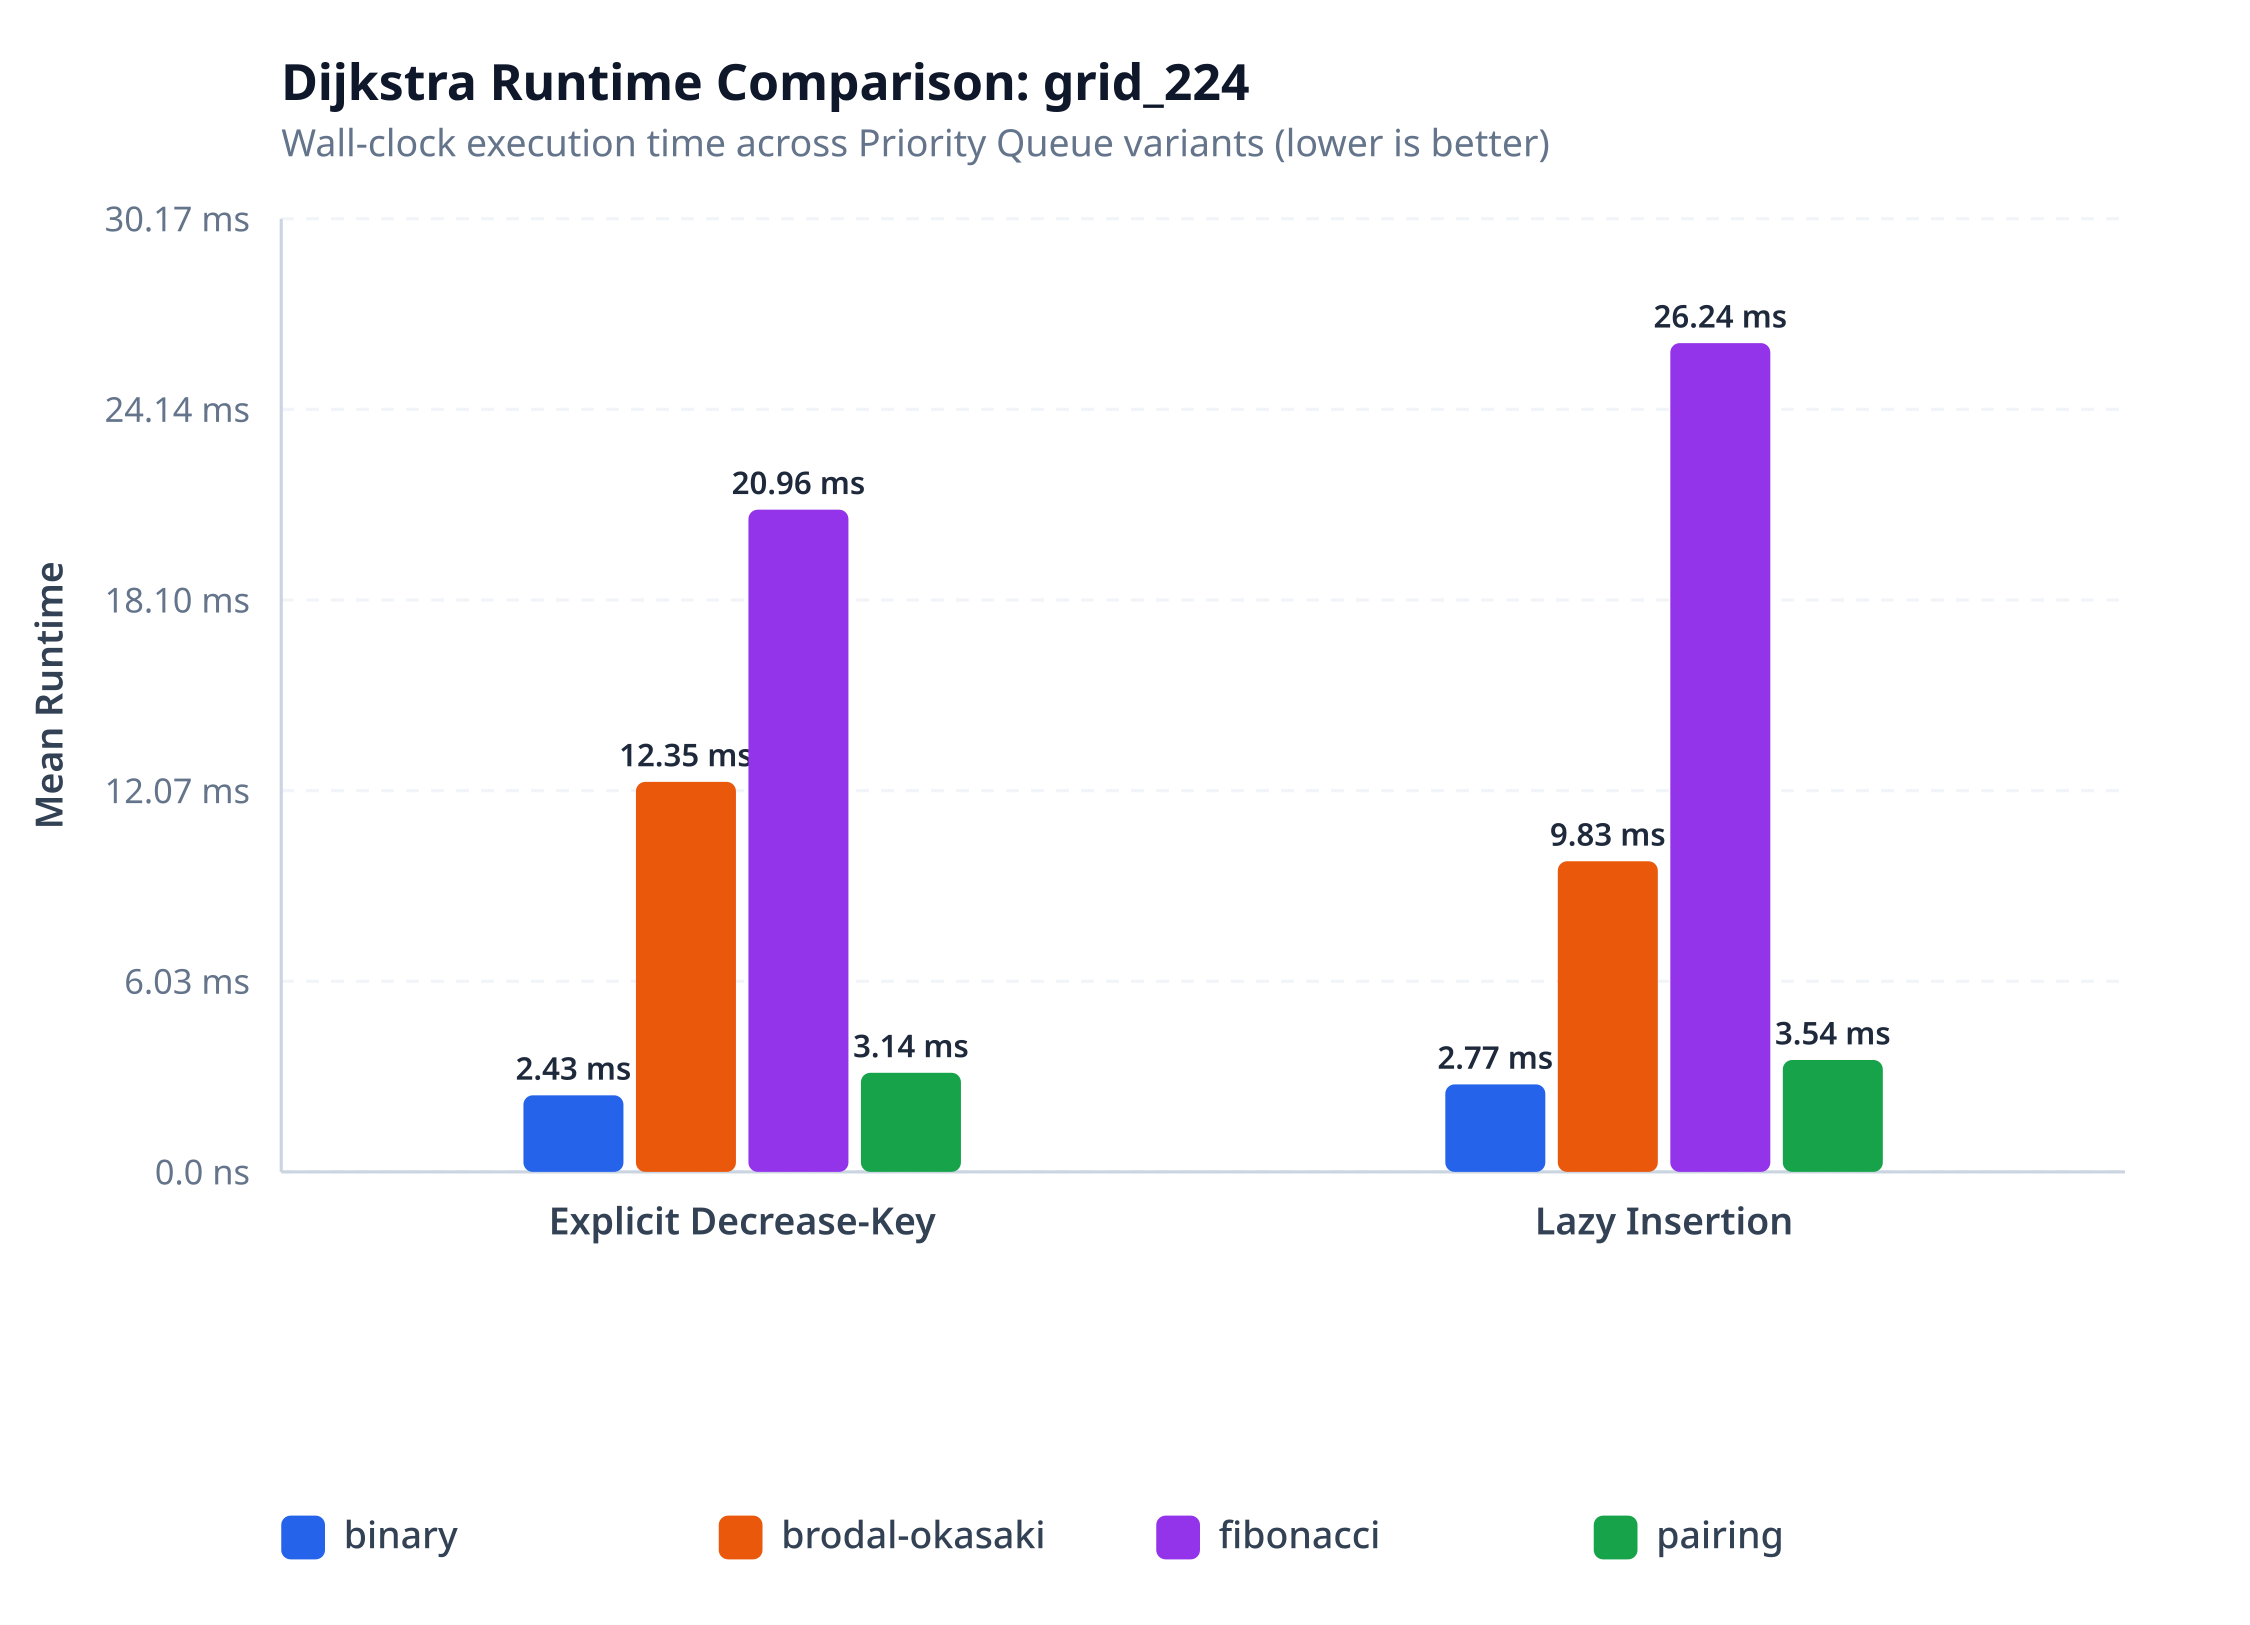
\includegraphics[width=0.48\textwidth]
    {frozen_results/figures/report_charts/runtime/grid_224.png}
  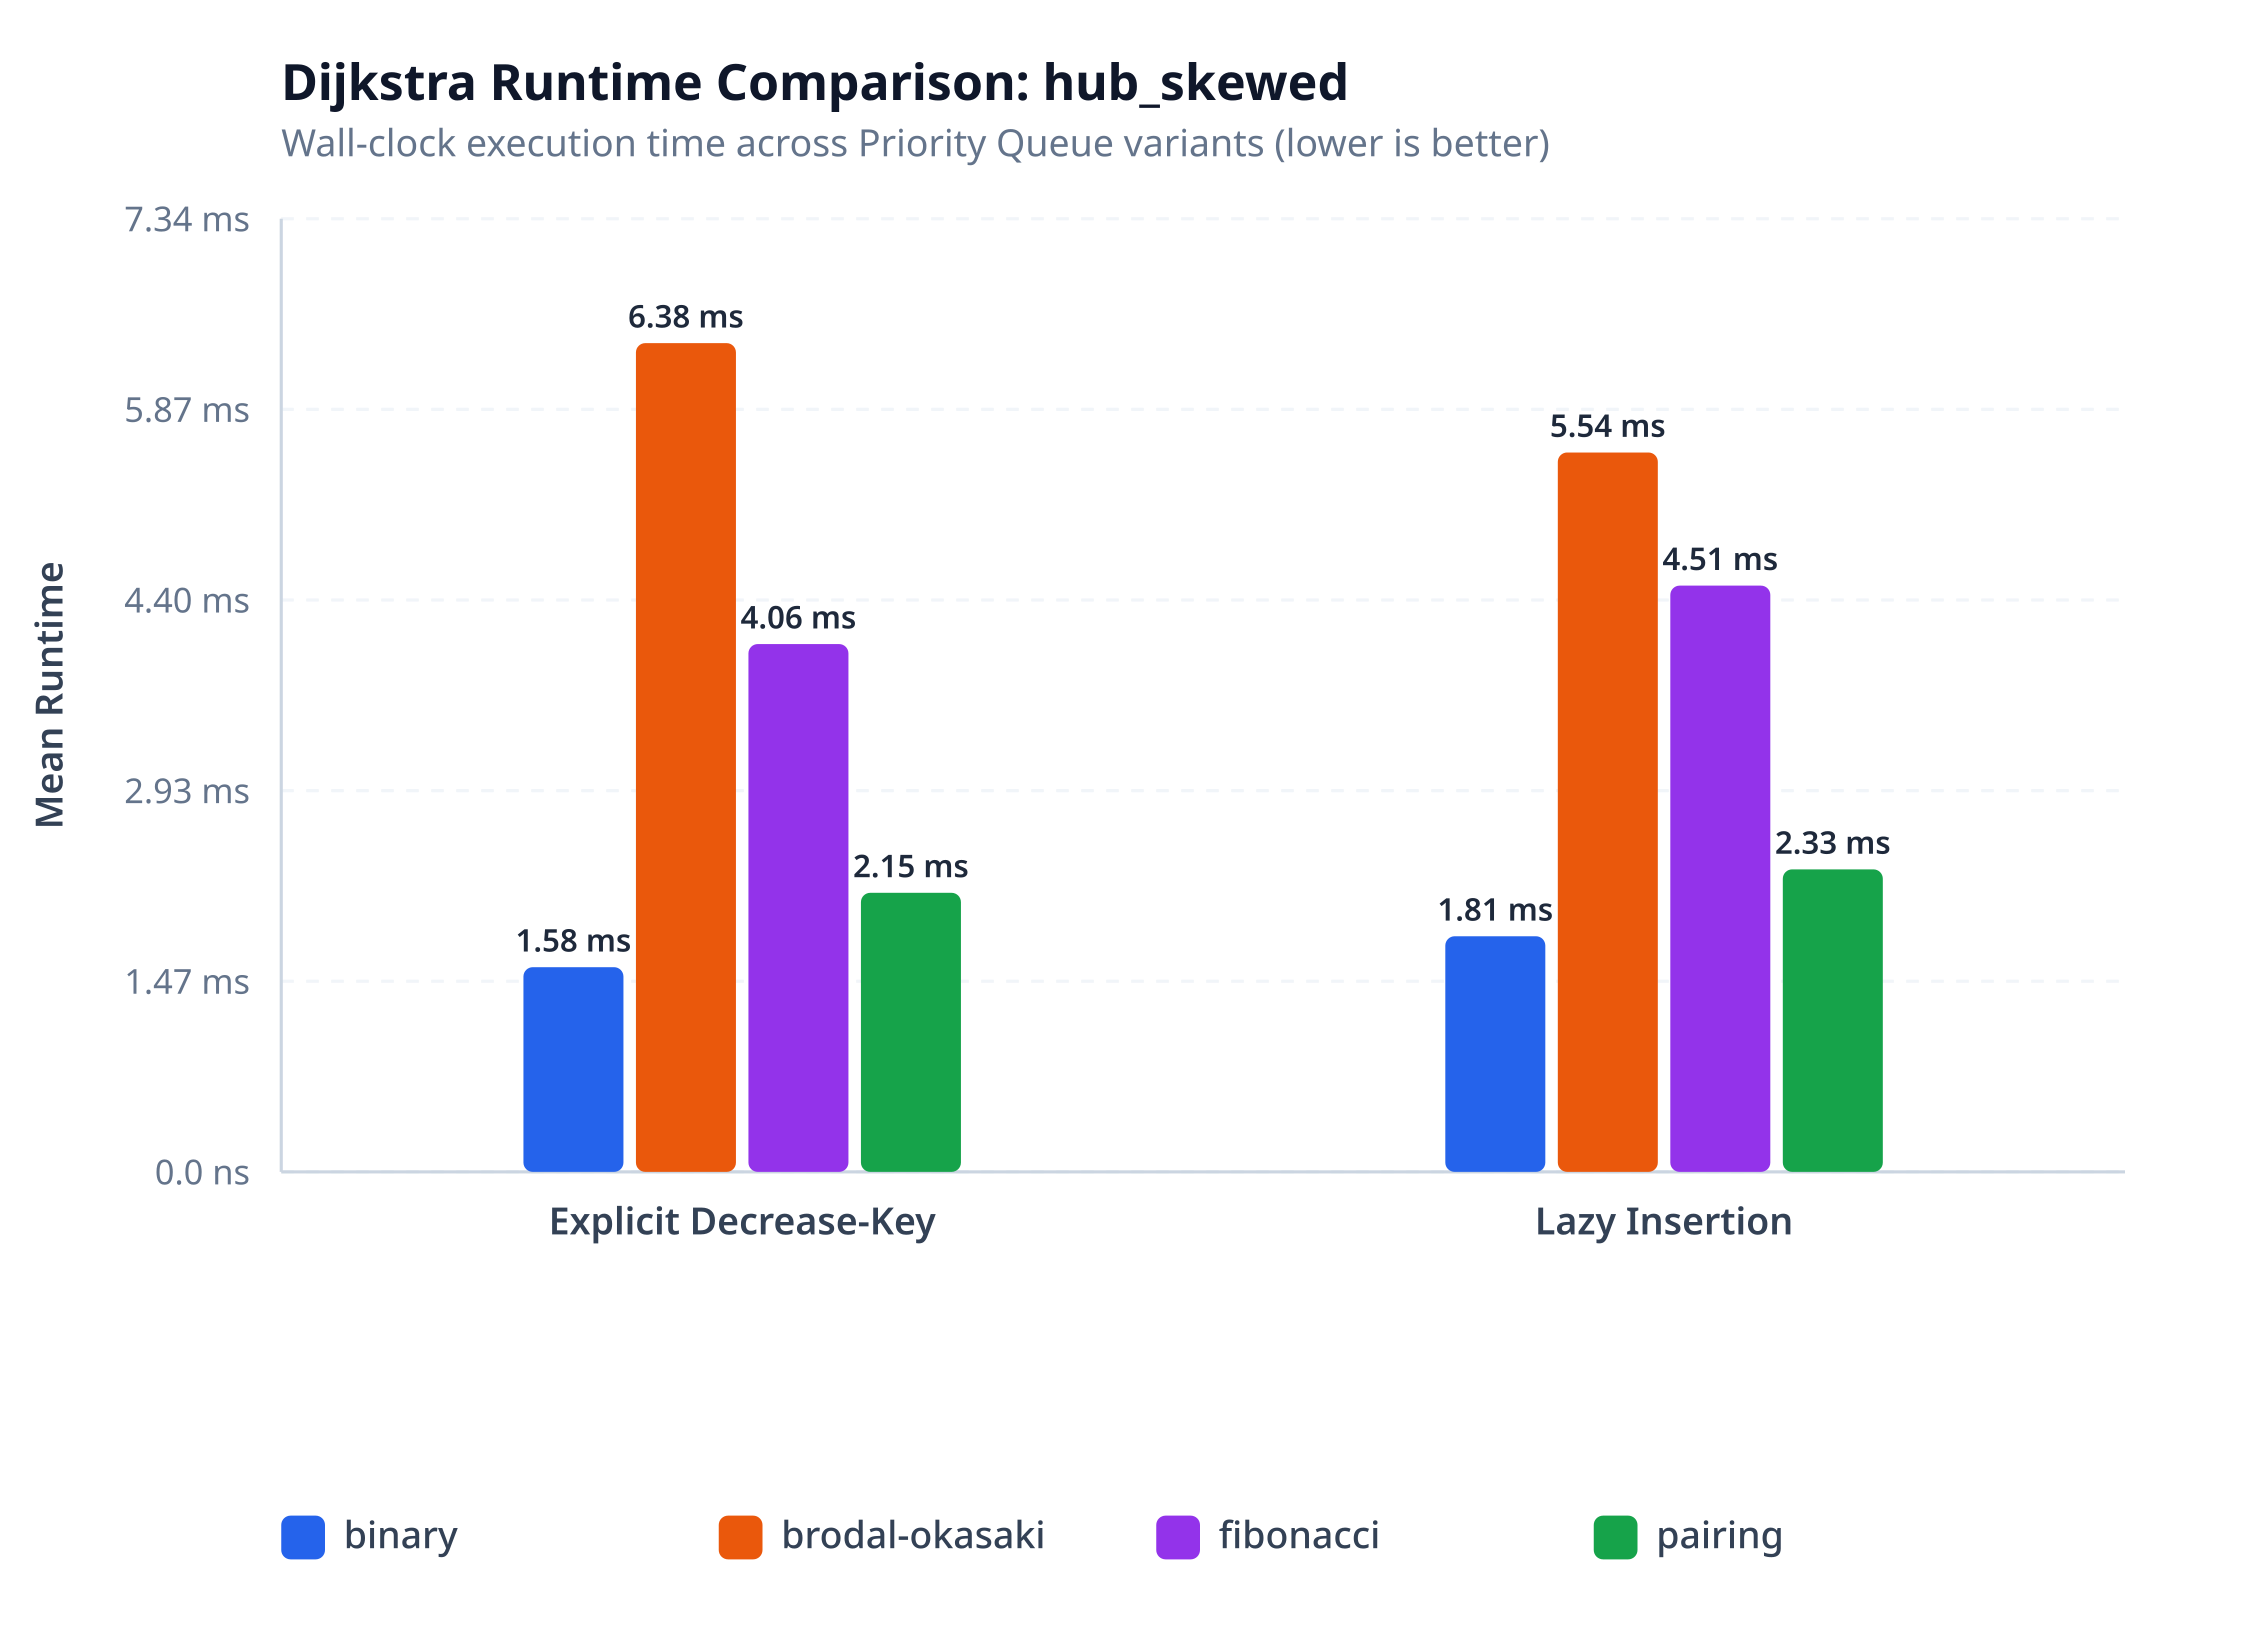
\includegraphics[width=0.48\textwidth]
    {frozen_results/figures/report_charts/runtime/hub_skewed.png}

  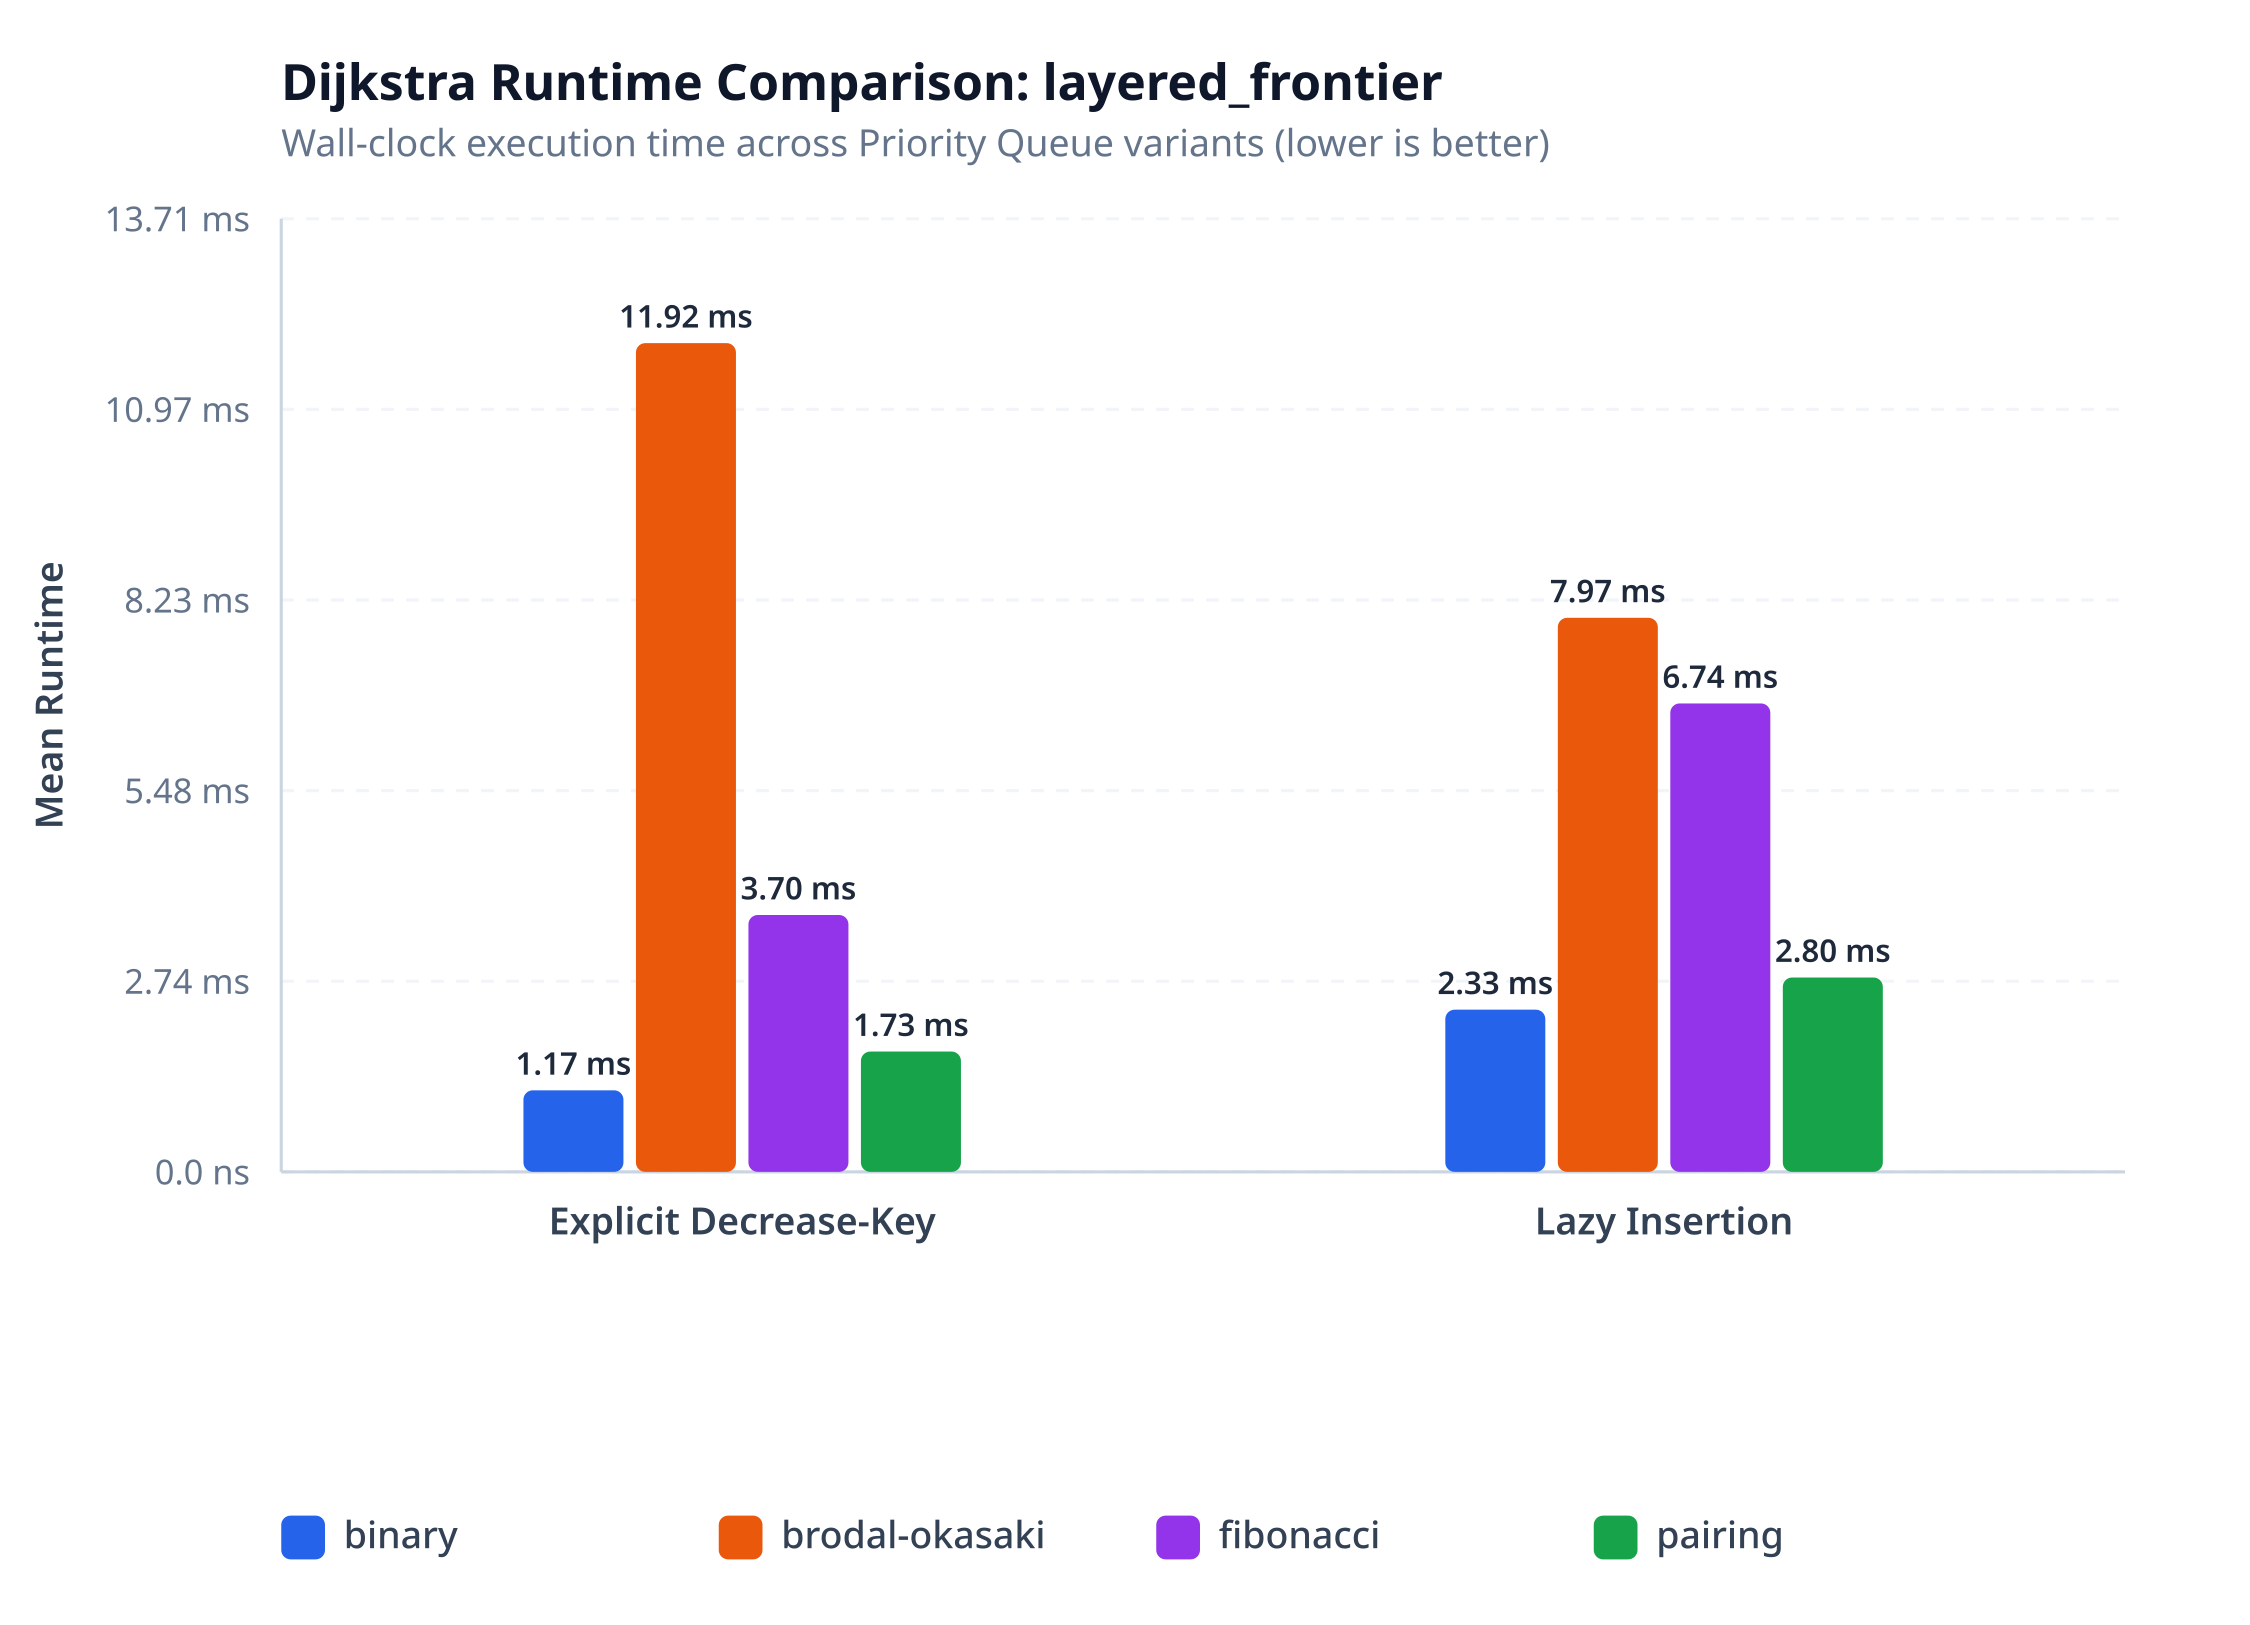
\includegraphics[width=0.48\textwidth]
    {frozen_results/figures/report_charts/runtime/layered_frontier.png}

  \caption{Runtime comparison between the four heap implementations across
  the seven input graphs. Each plot shows both \code{decrease_key} and
  \code{lazy} Dijkstra.}
  \label{fig:runtime-heap-comparison}
\end{figure}

The binary heap is the fastest implementation in every graph configuration.
The pairing heap is consistently second, while the Fibonacci and
Brodal--Okasaki heaps are slower. This ordering is stable across both the
uniform random graphs and the structured grid, hub-skewed, and layered graphs.

% CHECK: the Fibonacci figures below are from the previous run. The current
% frozen Fibonacci runtimes were measured while the CPU was throttled to about
% 1.7 GHz (perf cycles / runtime) and must be rerun before these are updated.
For example, on \code{uniform_dense} with \code{decrease_key}, the binary
heap takes approximately $1.63$~ms, compared with $2.15$~ms for the pairing
heap, $2.86$~ms for the Fibonacci heap, and $15.61$~ms for the
Brodal--Okasaki heap. On \code{grid_224}, the corresponding times are
approximately $2.43$~ms, $3.14$~ms, $7.24$~ms, and $12.35$~ms.

The binary heap's advantage is consistent with its contiguous array layout,
direct index-based navigation, and low constant factors. Although the
Fibonacci and Brodal--Okasaki heaps offer stronger theoretical bounds for some
priority-queue operations, their additional pointer manipulation and
bookkeeping do not translate into lower end-to-end Dijkstra runtime in these
experiments. The pairing heap is more competitive, but still remains slower
than the binary heap on every input.

\subsubsection{Runtime Comparison Between Lazy and Decrease-Key Dijkstra}

The runtime difference between the two Dijkstra variants is shown in
Figure~\ref{fig:lazy-decrease-runtime}. The figure reports the ratio
$T_{\mathrm{lazy}}/T_{\mathrm{decrease\_key}}$; values above one indicate that
\code{decrease\_key} is faster, while values below one indicate that the lazy
variant is faster.

\begin{figure}[H]
  \centering
  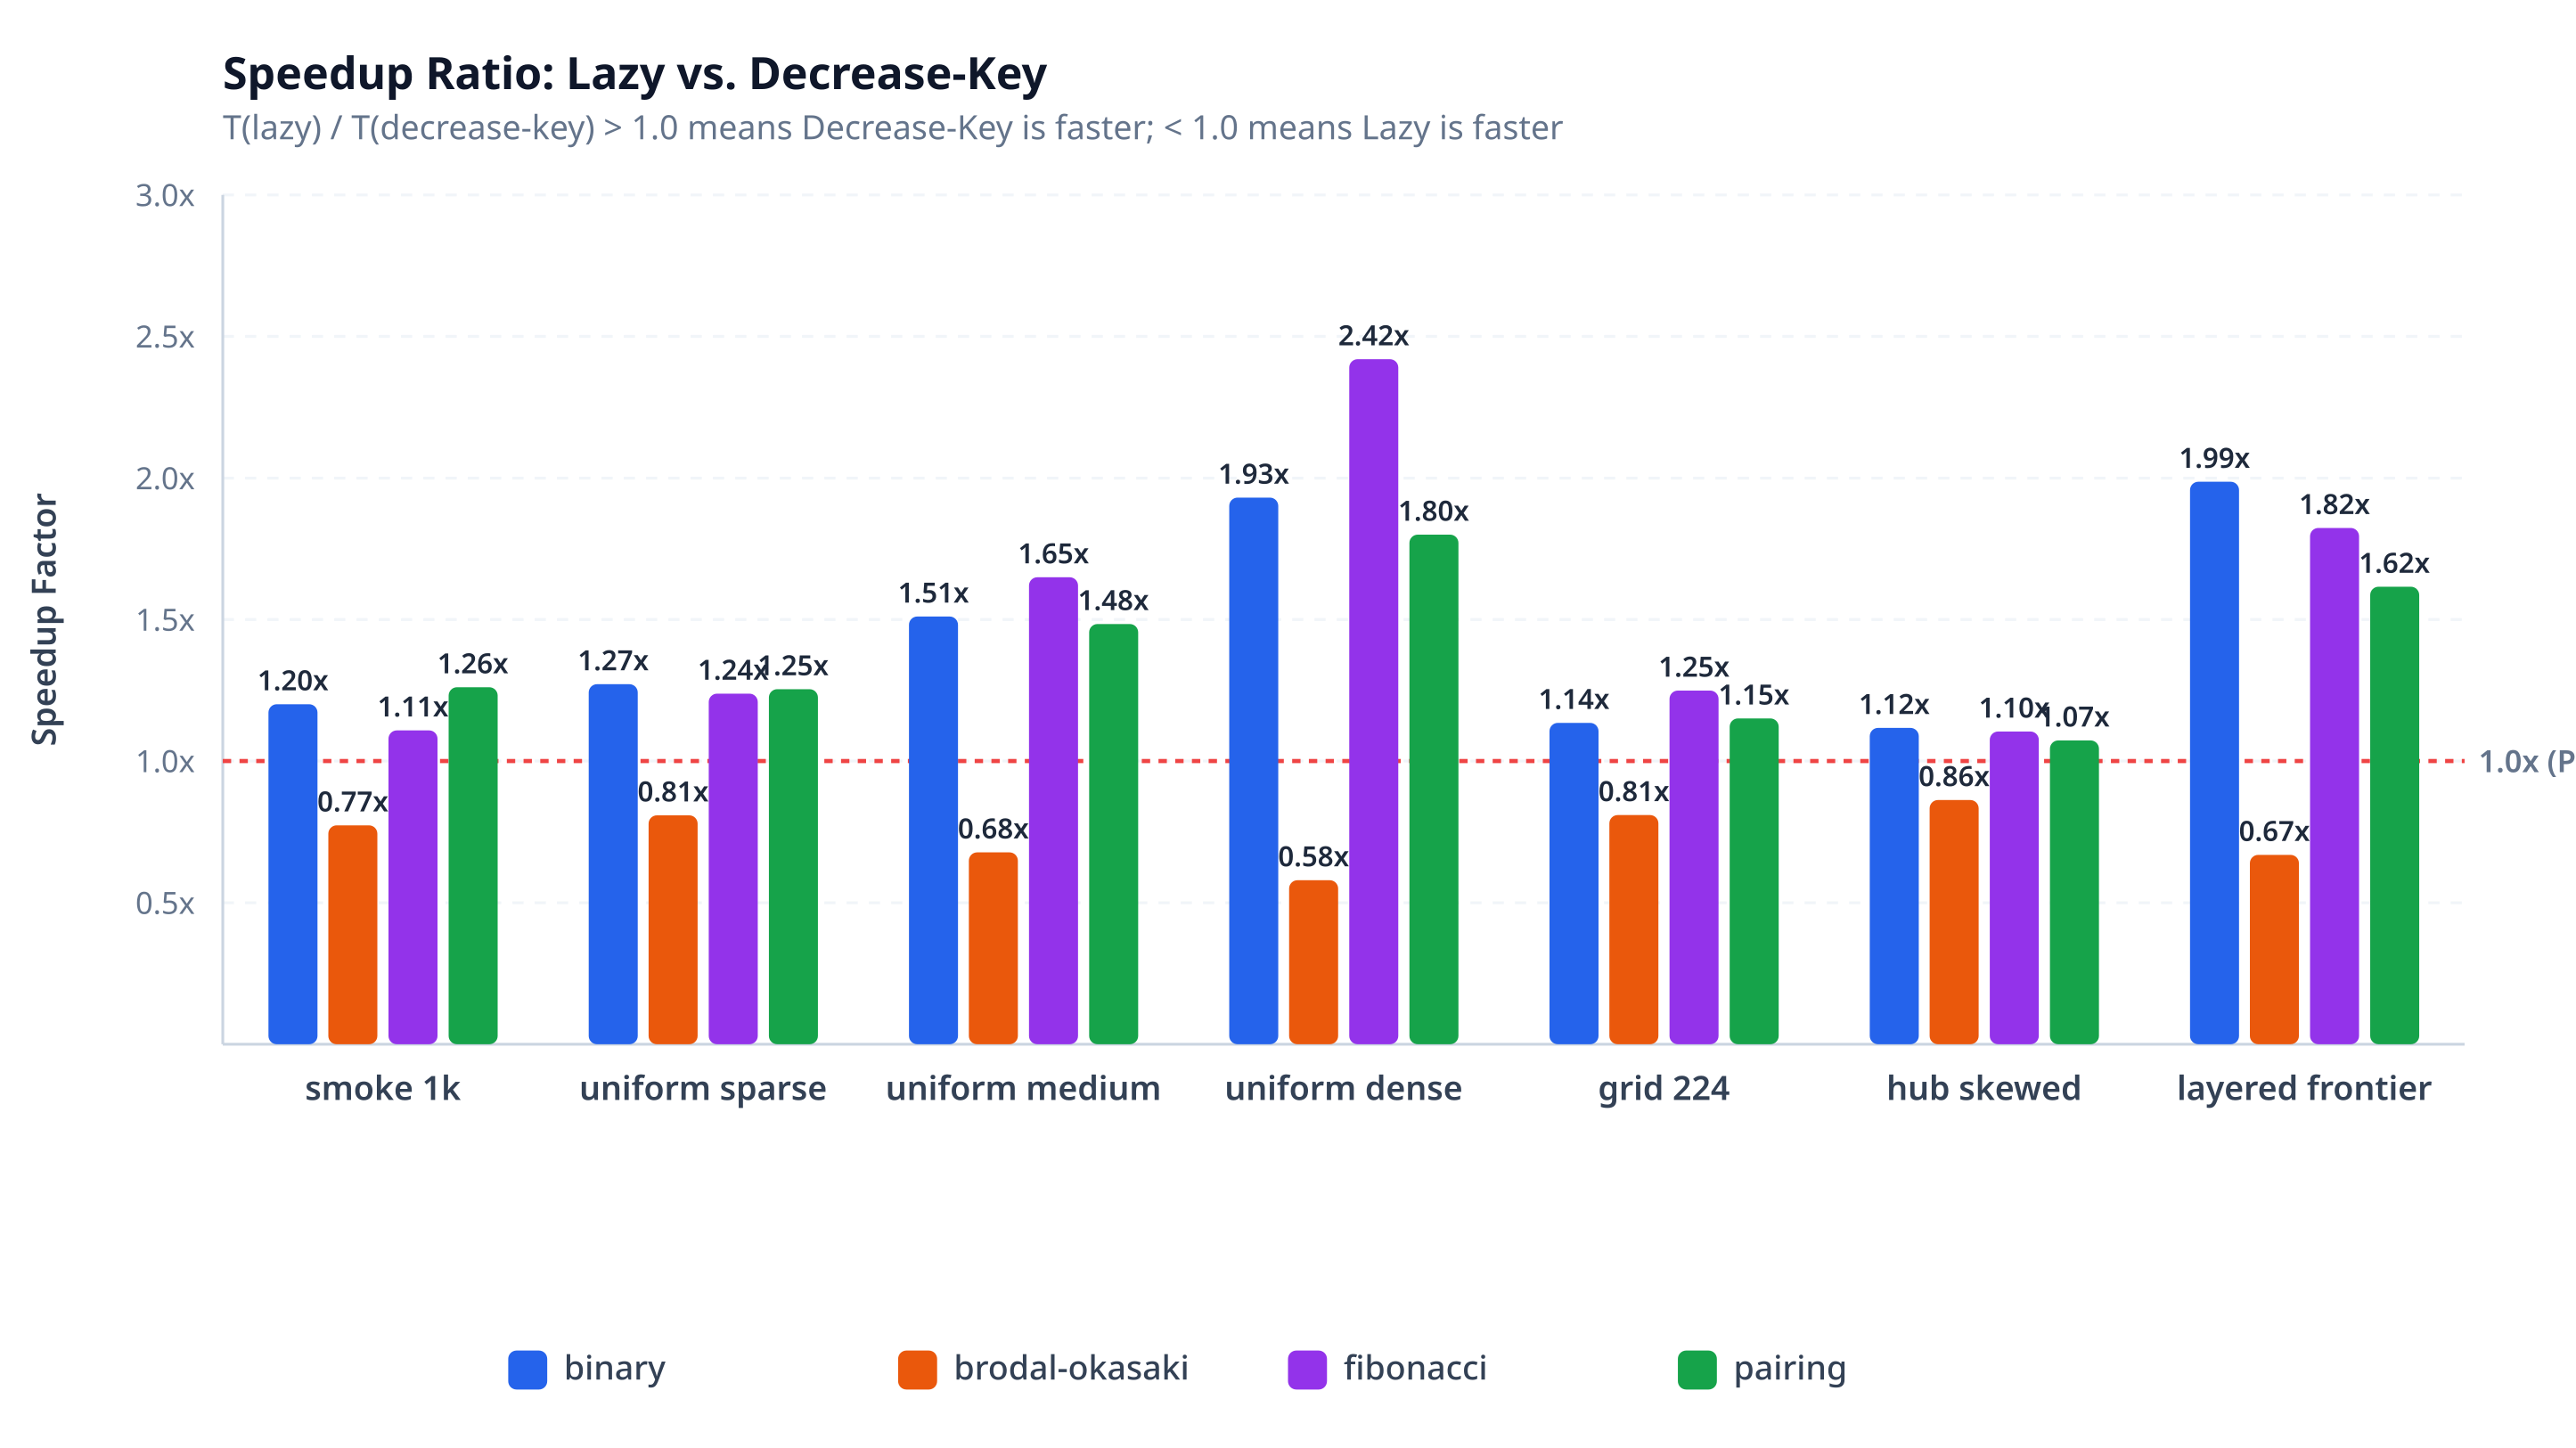
\includegraphics[width=0.95\textwidth]
    {frozen_results/figures/report_charts/runtime/lazy_vs_decrease_key.png}
  \caption{Runtime ratio between lazy and decrease-key Dijkstra. Values above
  one indicate that decrease-key is faster.}
  \label{fig:lazy-decrease-runtime}
\end{figure}

For the binary, pairing, and Fibonacci heaps, the \code{decrease\_key} variant
is faster on every graph. The difference is small on the sparse and
hub-skewed graphs, but becomes larger as the number of relaxations increases.
For example, with the binary heap, lazy processing is approximately $1.21$
times slower on \code{uniform_sparse}, $1.47$ times slower on
\code{uniform_medium}, and $1.85$ times slower on
\code{uniform_dense}. The same pattern appears for the pairing and Fibonacci
heaps.

This behaviour is consistent with the lazy algorithm inserting duplicate
entries whenever a shorter path is found. These stale entries remain in the
priority queue until they are extracted and discarded, increasing the number
of queue operations. The effect is particularly visible on
\code{uniform_dense} and \code{layered_frontier}, where the larger number of
relaxations produces a larger queue workload.

The Brodal--Okasaki implementation shows the opposite result. Its lazy
variant is faster on all seven graphs, with the largest relative improvements
on \code{uniform_dense}, \code{uniform_medium}, and
\code{layered_frontier}. For example, on \code{uniform_dense}, lazy
processing takes approximately $9.10$~ms compared with $15.61$~ms for
\code{decrease_key}. This result is specific to the current implementation:
the decrease-key operation requires additional tree-search and bookkeeping
work, whereas the lazy variant avoids those updates at the cost of processing
stale entries.

Overall, the results show that lazy processing is not uniformly inferior.
For the binary, pairing, and Fibonacci heaps, explicitly maintaining
decrease-key handles is beneficial, especially on denser graphs. For the
Brodal--Okasaki implementation, avoiding decrease-key operations is
consistently advantageous. Thus, the effect of the Dijkstra variant depends
not only on graph density and structure, but also on how efficiently each heap
implements decrease-key.

\subsection{Hardware Performance Results}

The hardware counters were collected with Linux \code{perf}, counting only the
timed Dijkstra loop (Section~3.1). Because the graphs range from 1,000 to
50,176 vertices, the figures below divide each count by the number of vertices
in the graph, which puts every graph on one axis while keeping the quantity
proportional to its cost.

\subsubsection{Work and Execution Efficiency}

\begin{figure}[H]
  \centering
  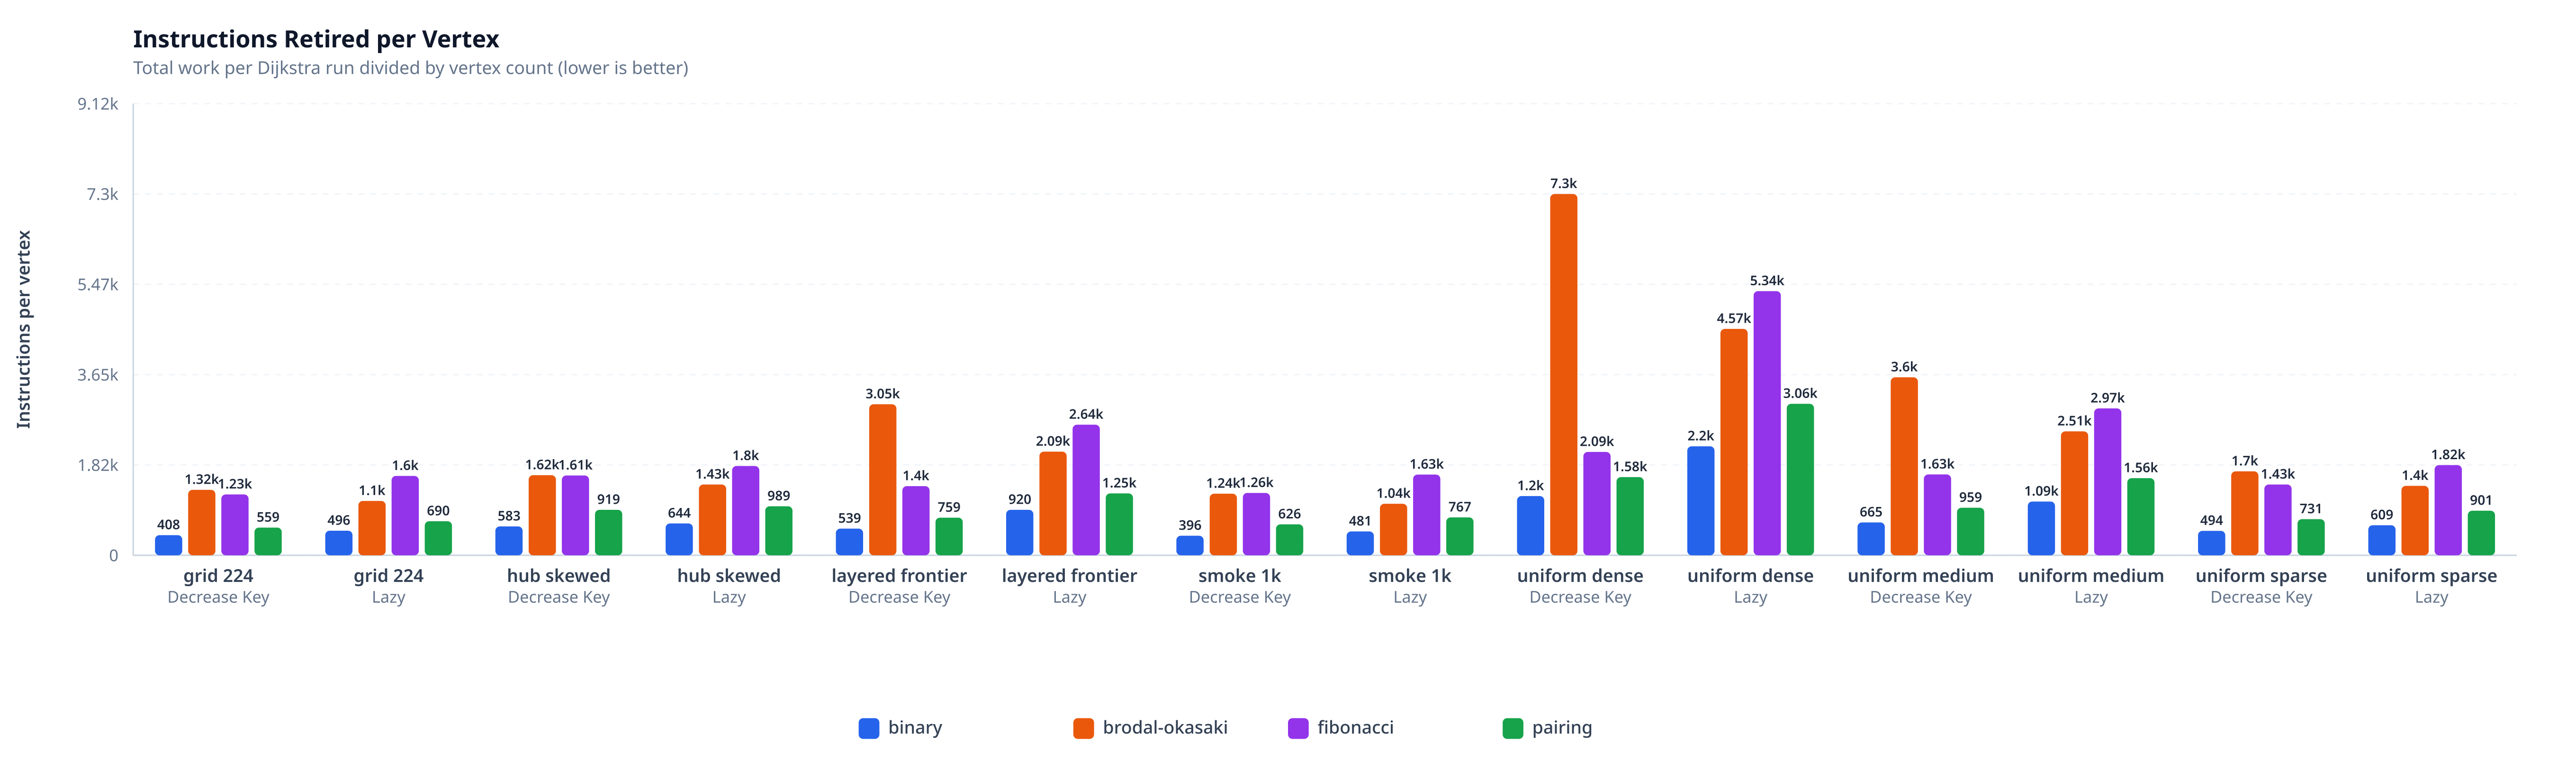
\includegraphics[width=0.95\textwidth]
    {frozen_results/figures/report_charts/perf/instructions_per_vertex.png}
  \caption{Instructions retired per vertex across heaps, input graphs, and
  Dijkstra variants.}
  \label{fig:instructions-per-vertex}
\end{figure}

\begin{figure}[H]
  \centering
  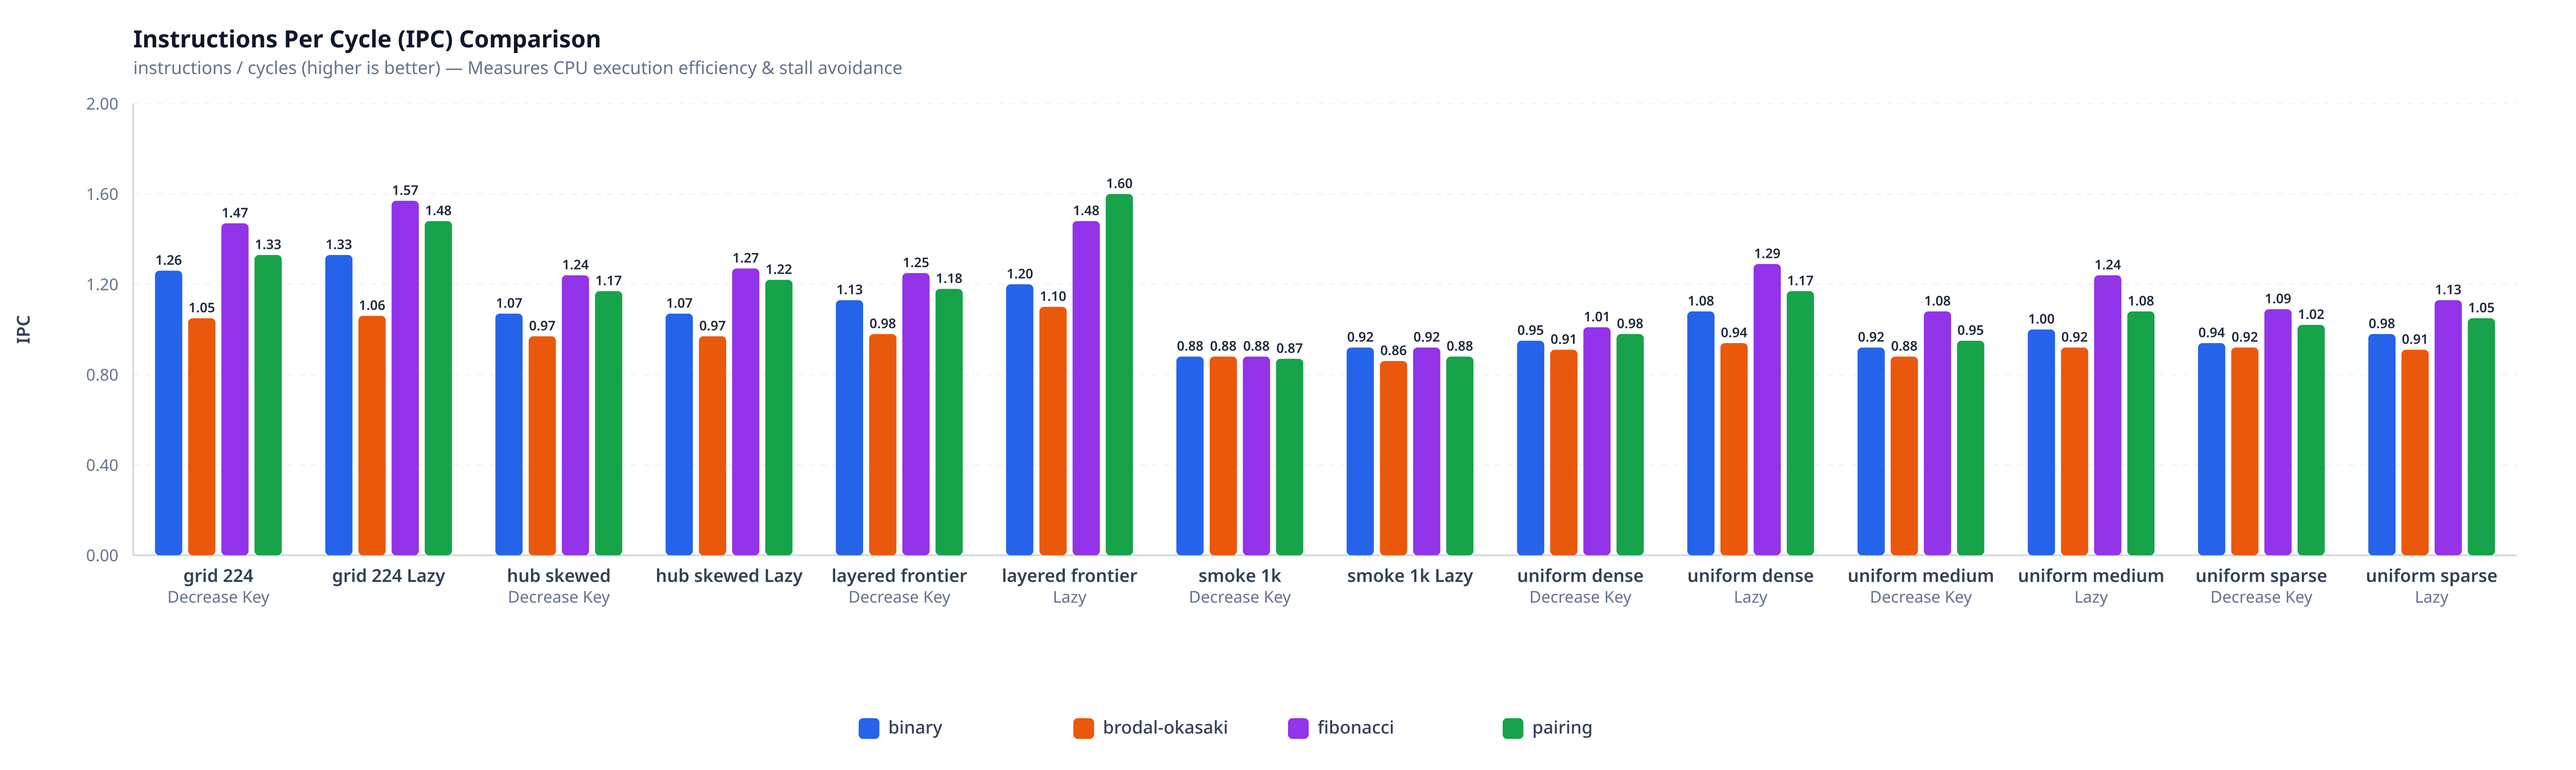
\includegraphics[width=0.95\textwidth]
    {frozen_results/figures/report_charts/perf/ipc_comparison.png}
  \caption{Instructions per cycle across heaps, input graphs, and Dijkstra
  variants.}
  \label{fig:ipc-comparison}
\end{figure}

\begin{figure}[H]
  \centering
  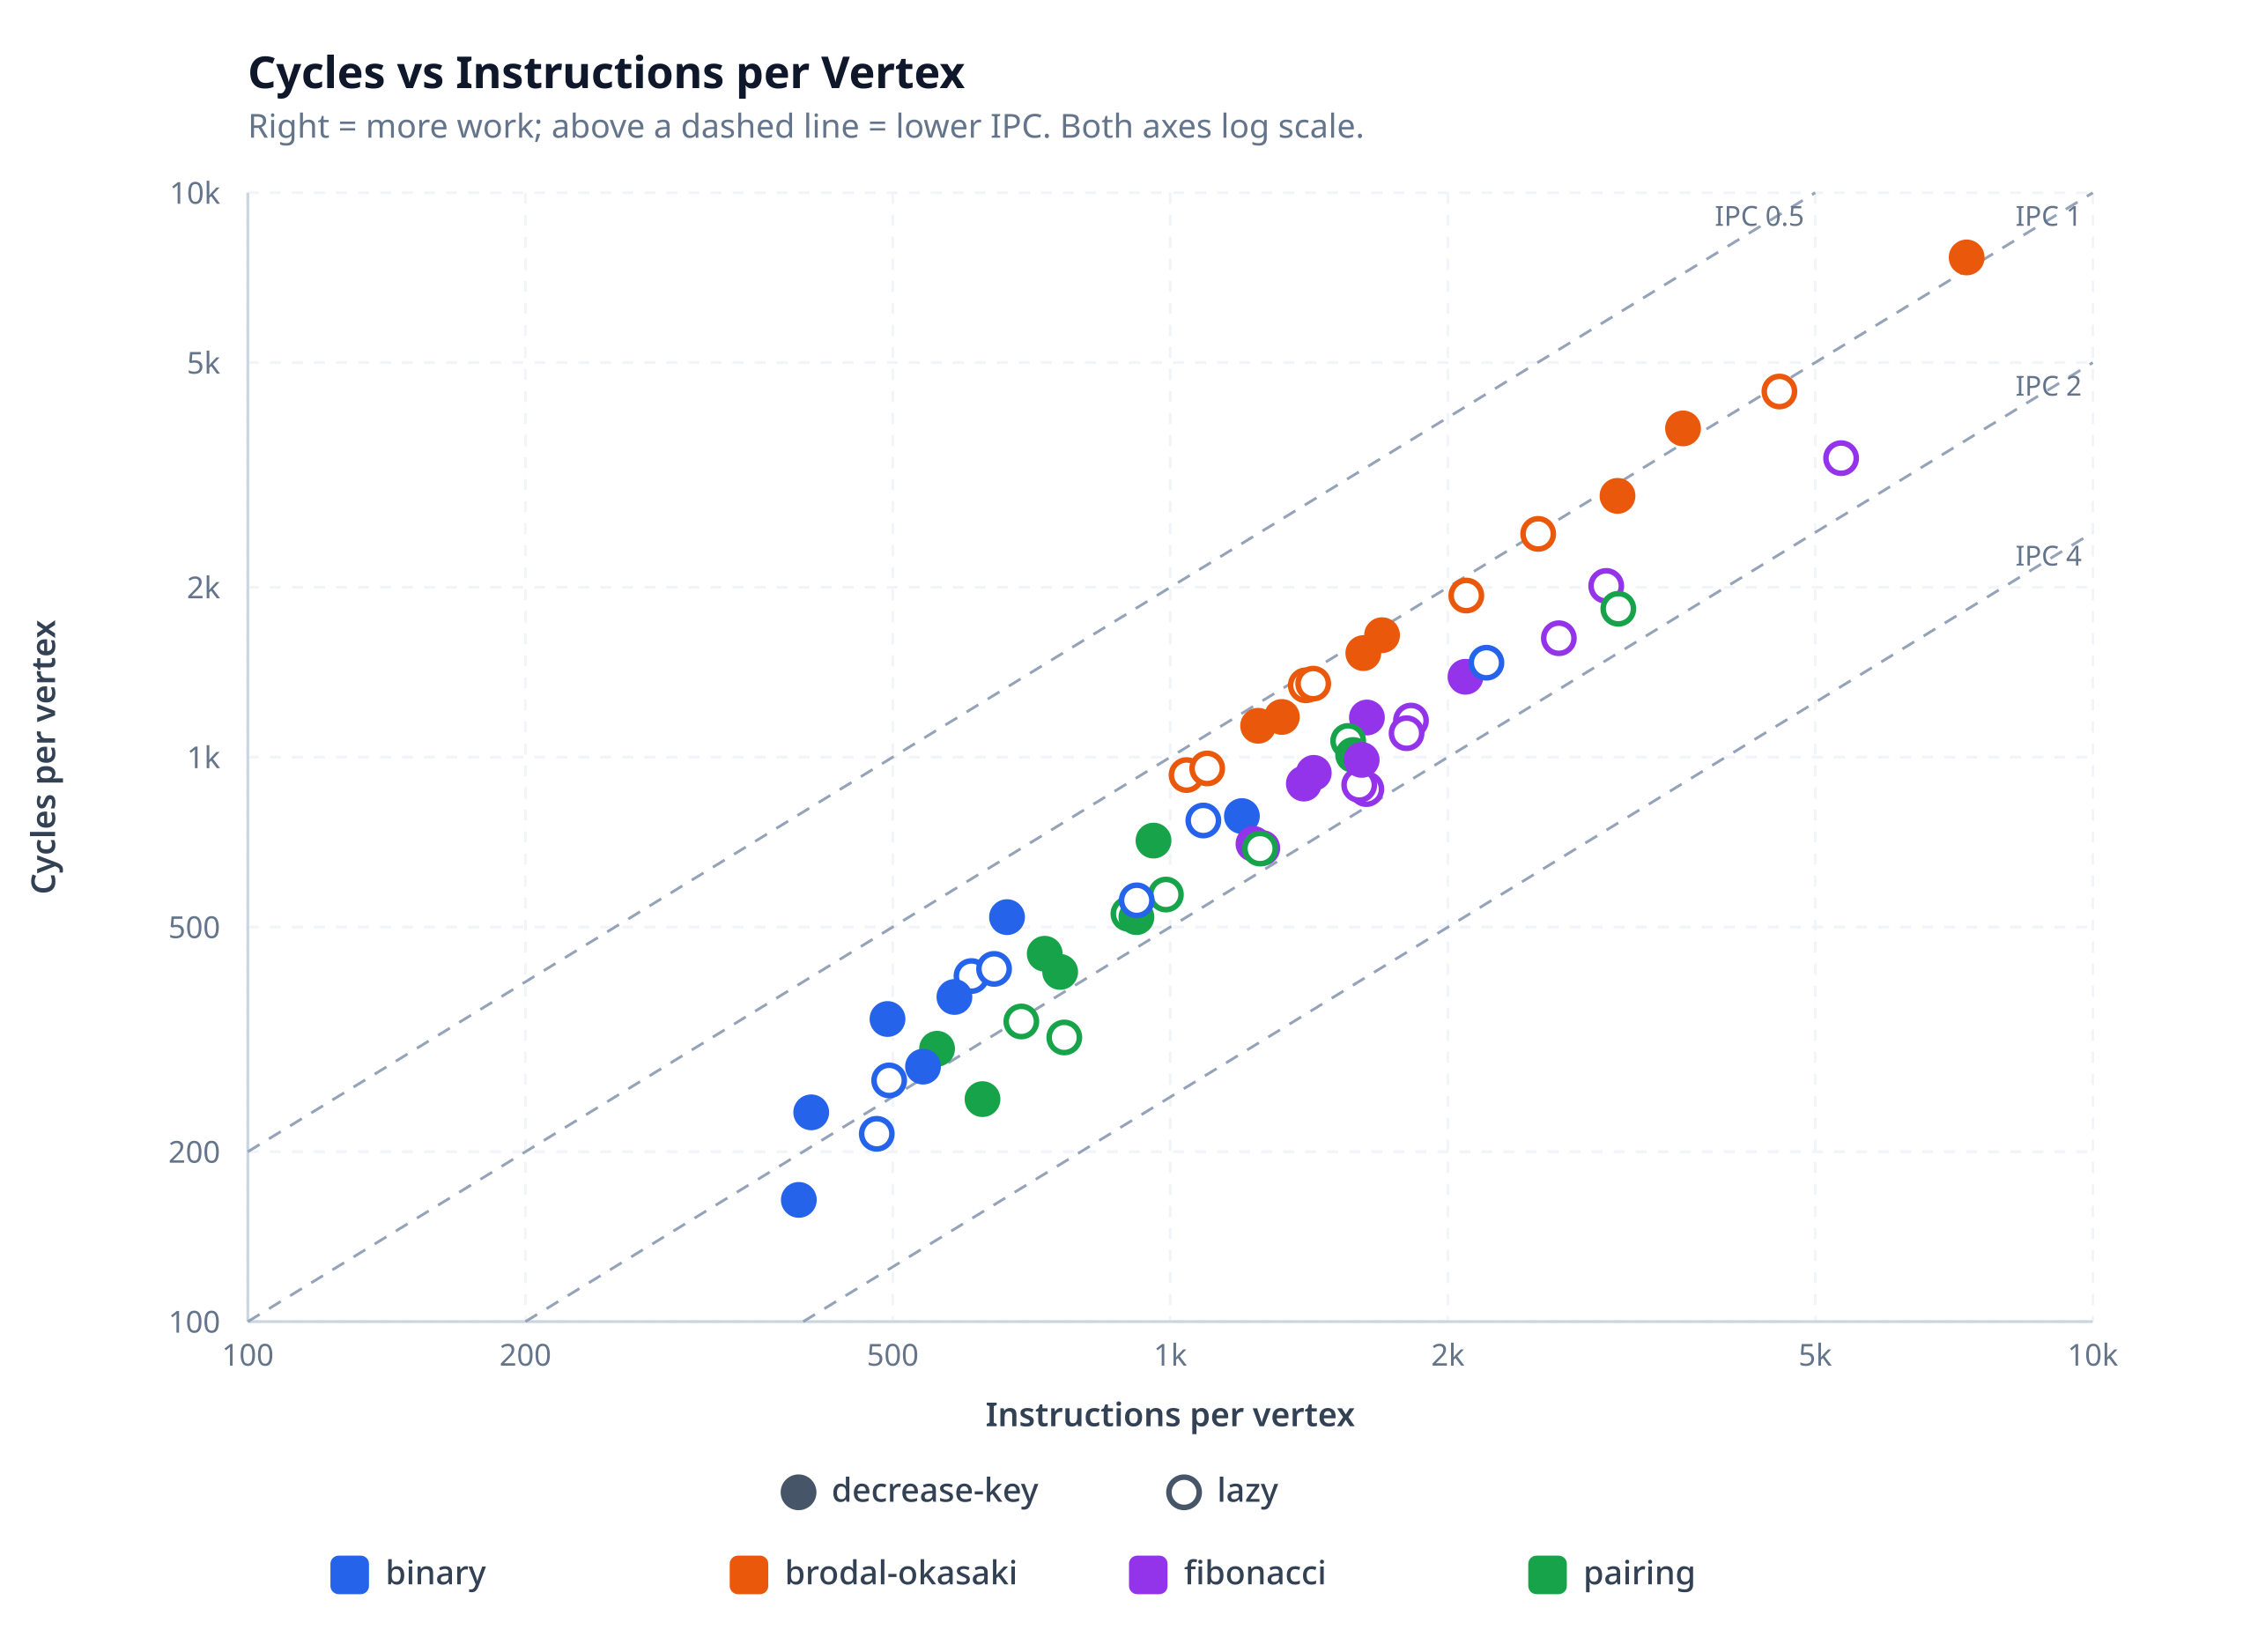
\includegraphics[width=0.6\textwidth]
    {frozen_results/figures/report_charts/perf/cycles_vs_instructions.png}
  \caption{Cycles against instructions per vertex (log scales). Points further
  right do more work; points above a dashed line execute it at a lower IPC.}
  \label{fig:cycles-vs-instructions}
\end{figure}

The slower heaps do substantially more work.
Averaged across the seven graphs in \code{decrease_key} mode, the binary heap
retires $612$ instructions per vertex, compared with $876$ for the pairing heap
($1.4\times$), $1{,}521$ for the Fibonacci heap ($2.5\times$), and $2{,}833$ for
the Brodal-Okasaki heap ($4.6\times$)
(Figure~\ref{fig:instructions-per-vertex}). Lazy processing raises the count
for the binary, pairing, and Fibonacci heaps ($919$, $1{,}317$, and $2{,}543$),
matching their slower lazy runtimes, and lowers it for Brodal-Okasaki
($2{,}020$), matching its faster lazy runtime.

The binary, pairing, and Fibonacci heaps execute that work at a similar rate,
with an average IPC of $1.69$, $1.78$, and $1.60$ respectively
(Figure~\ref{fig:ipc-comparison}). Among these three, the runtime ranking is
therefore explained by the amount of work rather than by how efficiently the
processor executes it, which appears in Figure~\ref{fig:cycles-vs-instructions}
as these points lying along the same IPC band. Brodal-Okasaki is the exception:
its average IPC is $1.04$, so it both does more work and executes it less
efficiently. On \code{uniform_dense} with \code{decrease_key} it retires
$6.1\times$ the binary heap's instructions per vertex but spends $9.8\times$ its
cycles ($7{,}682$ against $786$).

These results do not support Hypothesis~2.2. The binary heap does execute the
fewest instructions, but by a factor of $1.4$ to $4.6$ rather than orders of
magnitude, and its IPC is not systematically lower than that of the
pointer-based heaps: it is slightly below the pairing heap's and above the
Fibonacci and Brodal-Okasaki heaps'.

\subsubsection{Cache and Branch Behaviour}

\begin{figure}[H]
  \centering
  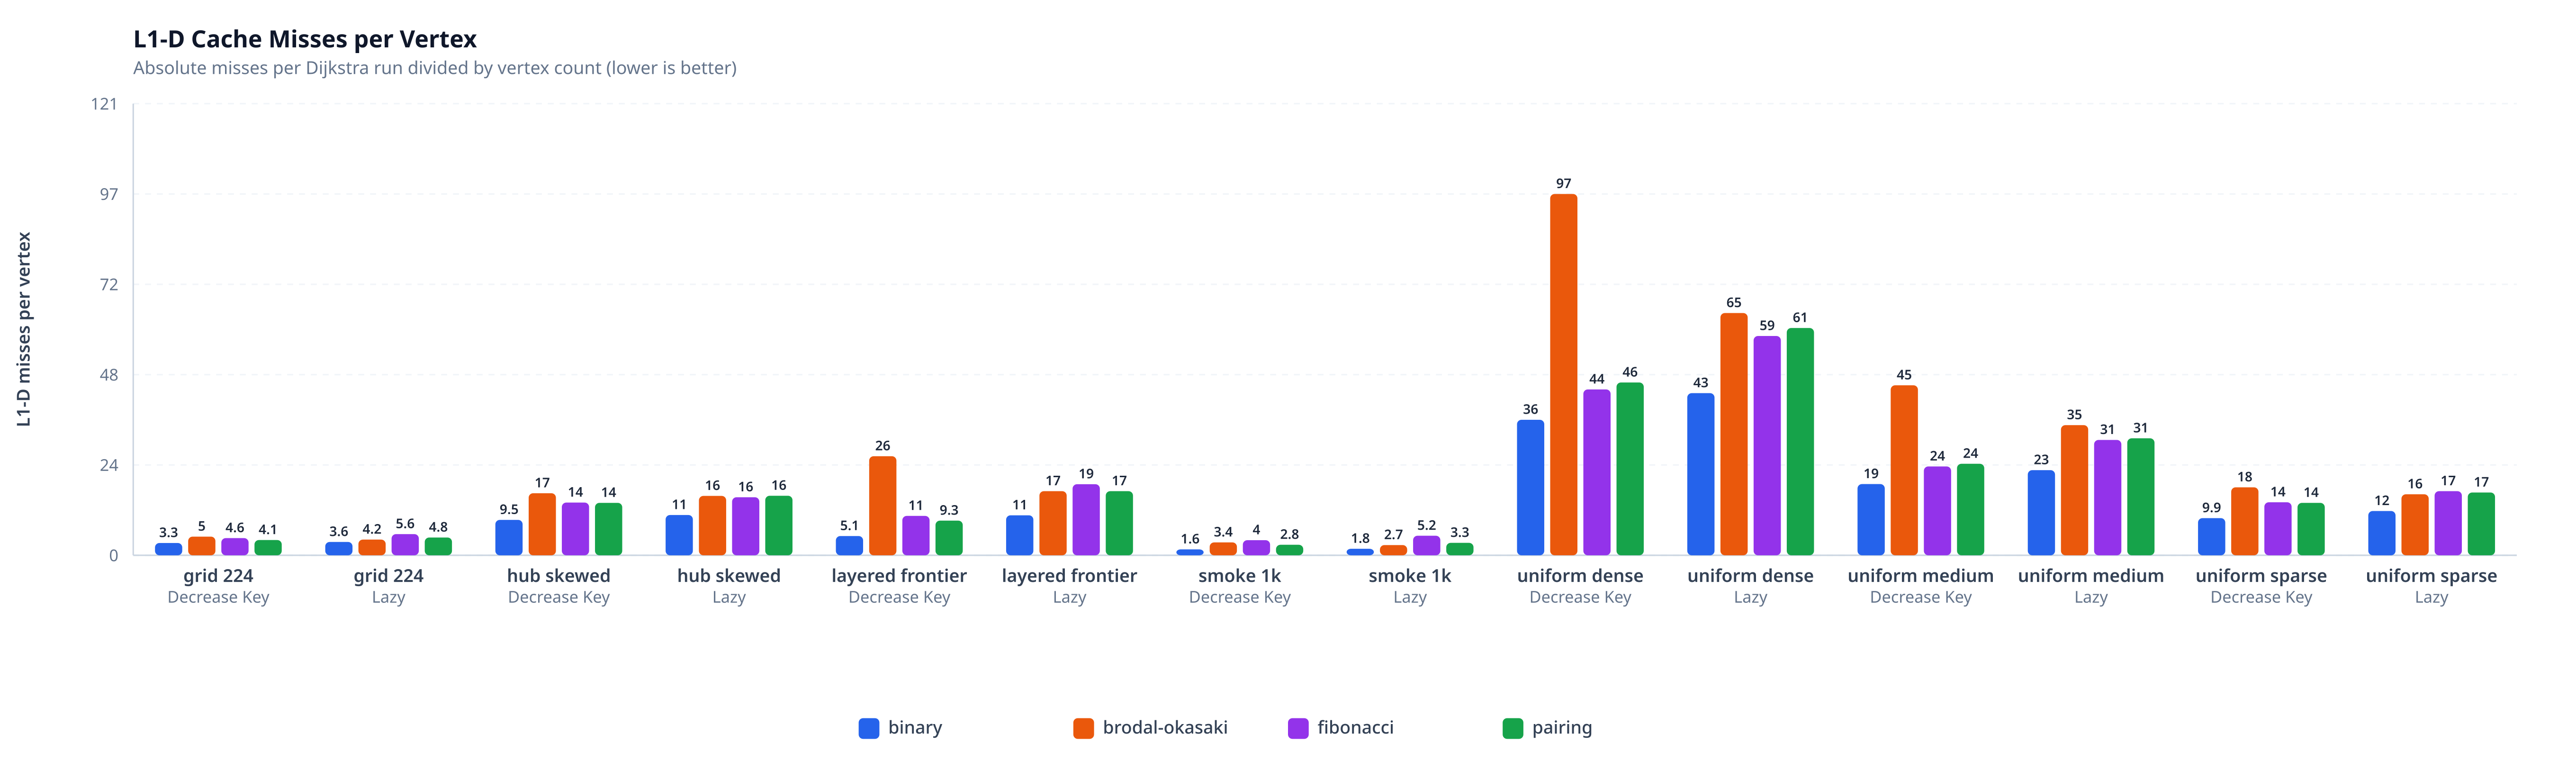
\includegraphics[width=0.95\textwidth]
    {frozen_results/figures/report_charts/perf/l1_misses_per_vertex.png}
  \caption{L1 data-cache misses per vertex across heaps, input graphs, and
  Dijkstra variants.}
  \label{fig:l1-misses-per-vertex}
\end{figure}

\begin{figure}[H]
  \centering
  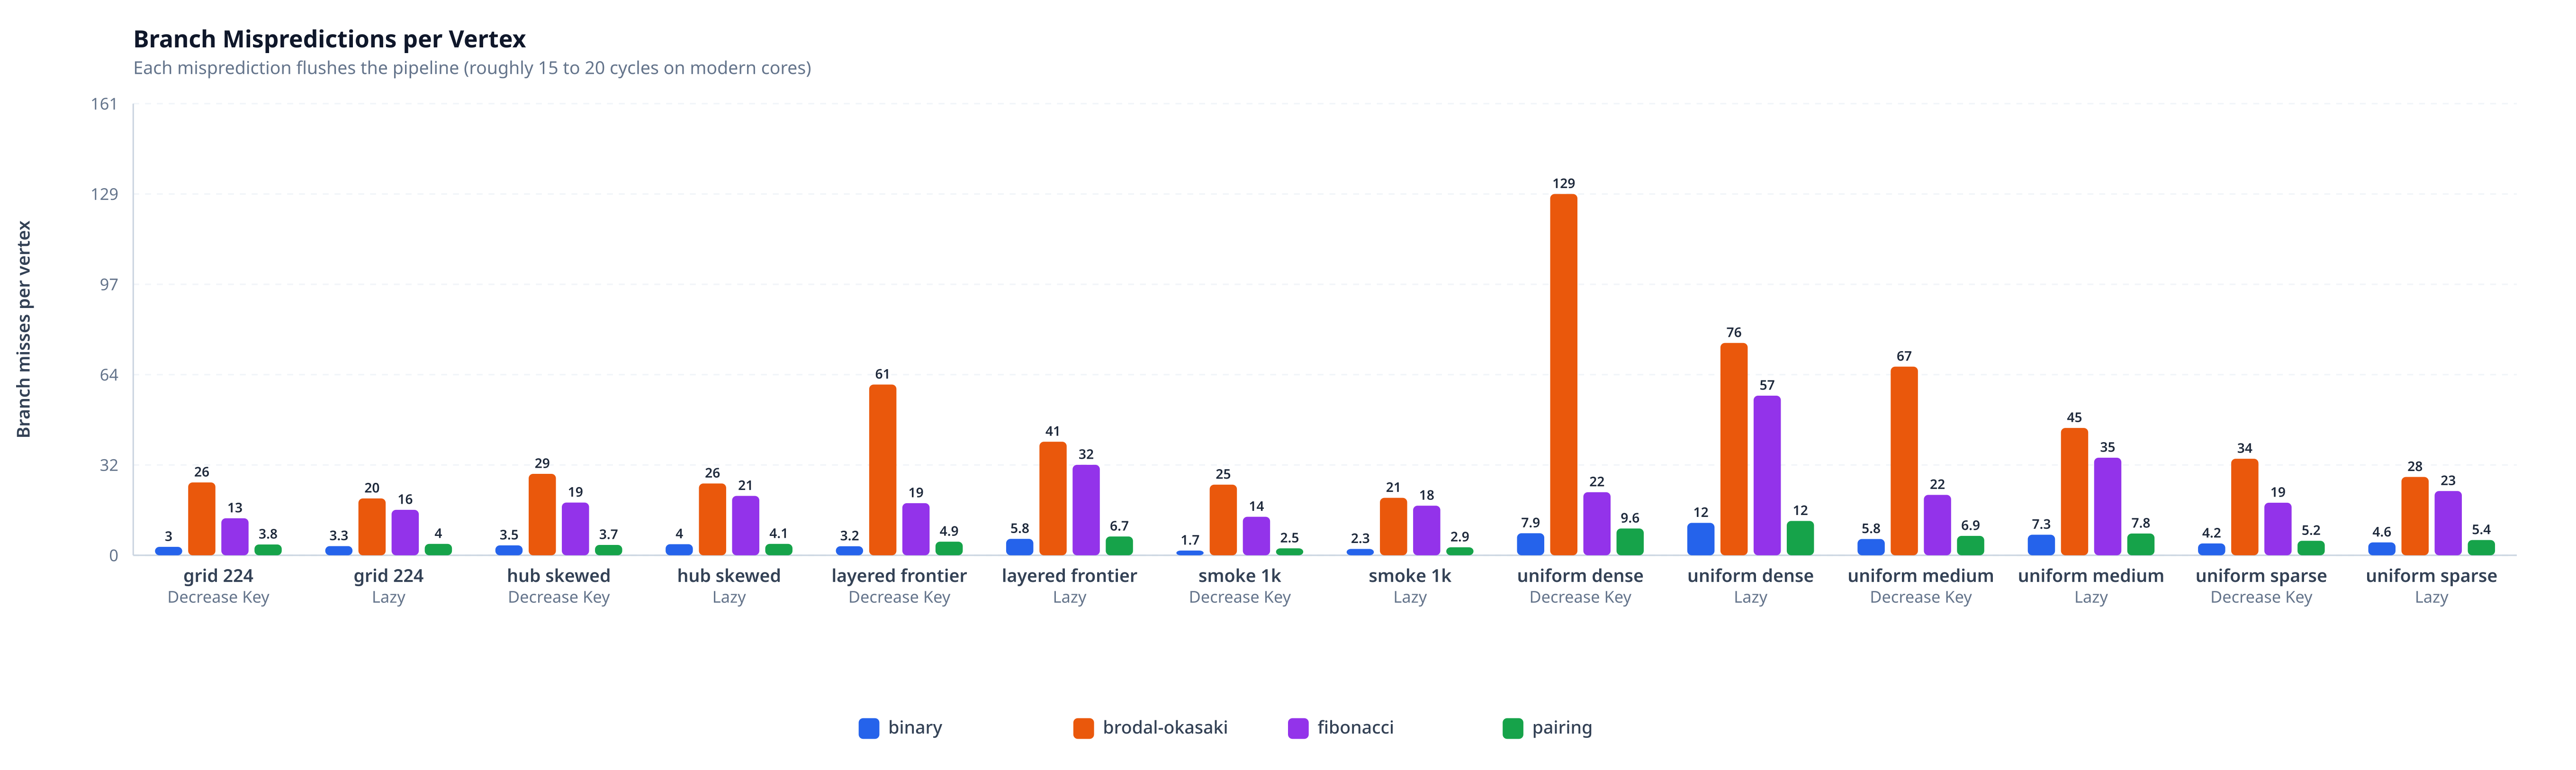
\includegraphics[width=0.95\textwidth]
    {frozen_results/figures/report_charts/perf/branch_misses_per_vertex.png}
  \caption{Branch mispredictions per vertex across heaps, input graphs, and
  Dijkstra variants.}
  \label{fig:branch-misses-per-vertex}
\end{figure}

\begin{figure}[H]
  \centering
  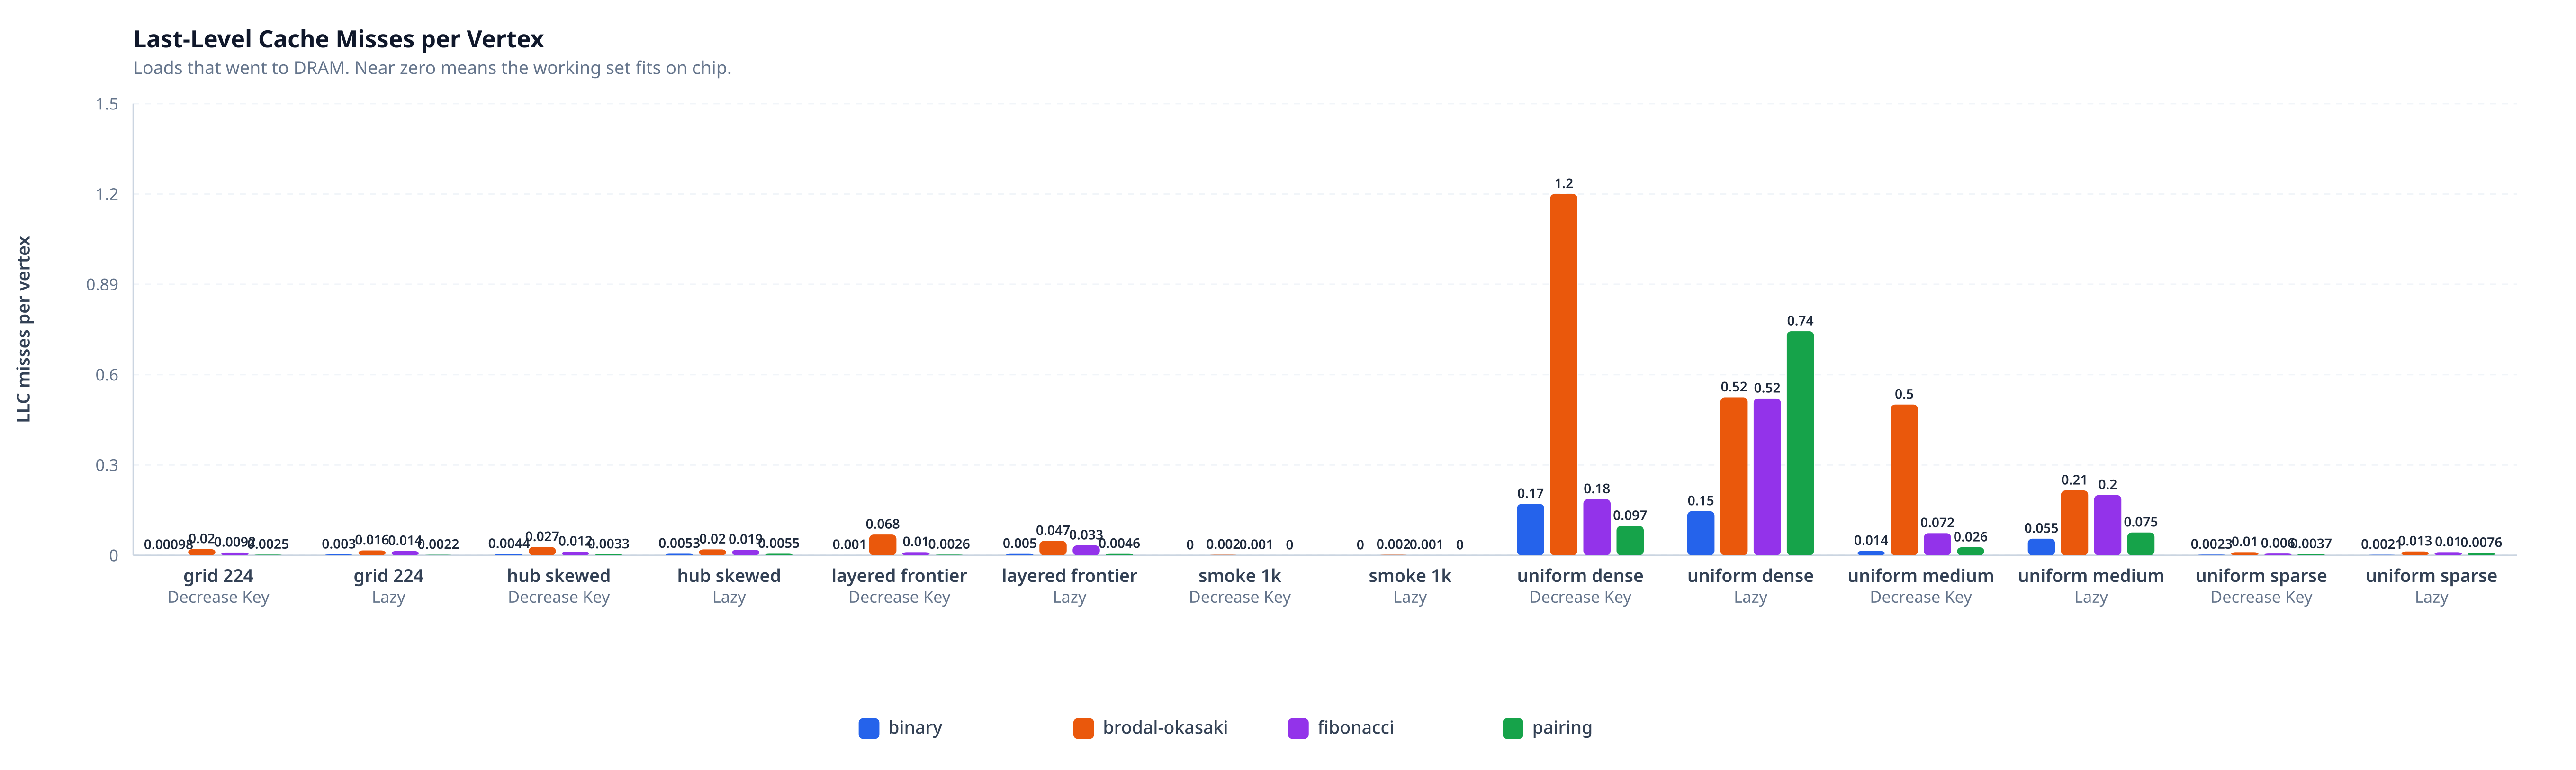
\includegraphics[width=0.95\textwidth]
    {frozen_results/figures/report_charts/perf/llc_misses_per_vertex.png}
  \caption{Last-level cache misses per vertex. Values near zero mean the
  working set stays on chip.}
  \label{fig:llc-misses-per-vertex}
\end{figure}

We report cache misses as counts rather than miss rates. A miss rate divides
misses by loads, and the number of loads differs widely between heaps, so a
heap that performs many extra loads that hit in the cache appears to have a
better rate while costing more. Measured as a rate, the binary heap has the
highest average L1 miss rate in \code{decrease_key} mode ($7.11\%$, against
$6.70\%$ for pairing, $4.54\%$ for Fibonacci, and $3.29\%$ for
Brodal-Okasaki), but it also performs the fewest loads ($147$ per vertex,
against $211$, $324$, and $763$). Counted per vertex, it has the fewest L1
misses: $12.2$, against $16.3$ for pairing, $16.5$ for Fibonacci, and $30.3$
for Brodal-Okasaki (Figure~\ref{fig:l1-misses-per-vertex}). This supports the
first part of Hypothesis~2.1, that the array layout gives the binary heap the
best cache behaviour, but not the predicted ordering of the pointer-based
heaps: the Fibonacci heap's larger nodes do not make it worse than the pairing
heap, and Brodal-Okasaki is the worst despite its contiguous buffer.

The cost of these misses is limited at our input sizes. Last-level cache
misses stay below one per vertex in every configuration and below $0.05$ in
47 of the 56 (Figure~\ref{fig:llc-misses-per-vertex}), so almost every L1 miss is
served from L2 or L3 rather than from main memory. The DRAM round-trips
anticipated in Hypothesis~2.1 therefore do not occur in these experiments; the
largest LLC counts appear on \code{uniform_dense}, whose working set is the
closest to the 12~MiB L3.

Branch mispredictions separate Brodal-Okasaki most clearly from the other
heaps (Figure~\ref{fig:branch-misses-per-vertex}). In \code{decrease_key}
mode it averages $53.3$ mispredictions per vertex ($10.8\%$ of branches),
against $4.2$ for the binary heap ($4.0\%$), $5.2$ for pairing ($3.3\%$), and
$18.2$ for Fibonacci ($5.2\%$). Its linking and cancellation code is driven by
data-dependent key comparisons, which the branch predictor cannot learn. At
the roughly 15 to 20 cycles each misprediction costs on modern cores, the
$129$ mispredictions per vertex on \code{uniform_dense} would account for
a quarter to a third of its $7{,}682$ cycles per vertex, which is consistent
with its low IPC.

\subsection{Memory Results}
\subsubsection{Peak Heap and Resident Memory}

Figures~\ref{fig:peak-heap-memory}
and~\ref{fig:peak-rss-memory} show the peak heap allocation and peak resident
set size recorded during the experiments.

% % Auto-generated by src/bench/bench2/plot2.py
\begin{table}[H]
  \centering
  \small
  \caption{Memory Footprint and Dynamic Allocator Pressure ($N=50{,}000$)}
  \label{tab:memory_footprint}
  \begin{tabular}{lllrrrrr}
    \toprule
    \textbf{Variant} & \textbf{Config} & \textbf{Mode} & \textbf{Peak Heap (KiB)} & \textbf{Peak RSS (MiB)} & \textbf{Mallocs} & \textbf{Frees} & \textbf{B/Vertex} \\
    \midrule
    binary & smoke_1k & Decr-Key & 23.5 & 50.0 & 3 & 3 & 24.0 \\
    brodal-okasaki & smoke_1k & Decr-Key & 39.1 & 50.0 & 2 & 2 & 40.1 \\
    fibonacci & smoke_1k & Decr-Key & 30.3 & 50.0 & 978 & 978 & 31.0 \\
    pairing & smoke_1k & Decr-Key & 24.2 & 49.9 & 978 & 978 & 24.8 \\
    binary & smoke_1k & Lazy & 23.5 & 50.0 & 3 & 3 & 24.0 \\
    brodal-okasaki & smoke_1k & Lazy & 39.1 & 50.0 & 2 & 2 & 40.1 \\
    fibonacci & smoke_1k & Lazy & 38.5 & 50.0 & 1,277 & 1,277 & 39.4 \\
    pairing & smoke_1k & Lazy & 29.8 & 50.0 & 1,282 & 1,282 & 30.5 \\
    \addlinespace
    binary & uniform_sparse & Decr-Key & 234.4 & 50.0 & 3 & 3 & 24.0 \\
    brodal-okasaki & uniform_sparse & Decr-Key & 390.7 & 50.2 & 2 & 2 & 40.0 \\
    fibonacci & uniform_sparse & Decr-Key & 300.1 & 50.2 & 9,782 & 9,782 & 30.7 \\
    pairing & uniform_sparse & Decr-Key & 236.7 & 50.2 & 9,782 & 9,782 & 24.2 \\
    binary & uniform_sparse & Lazy & 234.4 & 50.0 & 3 & 3 & 24.0 \\
    brodal-okasaki & uniform_sparse & Lazy & 390.7 & 50.3 & 2 & 2 & 40.0 \\
    fibonacci & uniform_sparse & Lazy & 372.5 & 50.4 & 12,824 & 12,824 & 38.1 \\
    pairing & uniform_sparse & Lazy & 289.2 & 50.3 & 12,848 & 12,848 & 29.6 \\
    \addlinespace
    binary & uniform_medium & Decr-Key & 468.8 & 50.3 & 3 & 3 & 24.0 \\
    brodal-okasaki & uniform_medium & Decr-Key & 3,840.1 & 52.2 & 4 & 4 & 196.6 \\
    fibonacci & uniform_medium & Decr-Key & 890.7 & 51.1 & 20,001 & 20,001 & 45.6 \\
    pairing & uniform_medium & Decr-Key & 681.2 & 50.8 & 20,001 & 20,001 & 34.9 \\
    binary & uniform_medium & Lazy & 1,093.8 & 50.8 & 5 & 5 & 56.0 \\
    brodal-okasaki & uniform_medium & Lazy & 2,061.3 & 51.3 & 3 & 3 & 105.5 \\
    fibonacci & uniform_medium & Lazy & 1,496.2 & 51.9 & 38,740 & 38,740 & 76.6 \\
    pairing & uniform_medium & Lazy & 1,113.3 & 51.6 & 38,765 & 38,765 & 57.0 \\
    \addlinespace
    binary & uniform_dense & Decr-Key & 234.4 & 50.1 & 3 & 3 & 24.0 \\
    brodal-okasaki & uniform_dense & Decr-Key & 3,840.1 & 53.9 & 5 & 5 & 393.2 \\
    fibonacci & uniform_dense & Decr-Key & 571.7 & 50.6 & 10,002 & 10,002 & 58.5 \\
    pairing & uniform_dense & Decr-Key & 430.4 & 50.5 & 10,002 & 10,002 & 44.1 \\
    binary & uniform_dense & Lazy & 1,093.8 & 50.8 & 7 & 7 & 112.0 \\
    brodal-okasaki & uniform_dense & Lazy & 1,920.1 & 51.5 & 4 & 4 & 196.6 \\
    fibonacci & uniform_dense & Lazy & 1,514.9 & 52.0 & 32,799 & 32,799 & 155.1 \\
    pairing & uniform_dense & Lazy & 1,104.8 & 51.5 & 32,816 & 32,816 & 113.1 \\
    \addlinespace
    binary & grid_224 & Decr-Key & 1,176.0 & 50.4 & 3 & 3 & 24.0 \\
    brodal-okasaki & grid_224 & Decr-Key & 1,960.1 & 52.0 & 2 & 2 & 40.0 \\
    fibonacci & grid_224 & Decr-Key & 416.6 & 50.4 & 50,178 & 50,178 & 8.5 \\
    pairing & grid_224 & Decr-Key & 409.6 & 50.4 & 50,178 & 50,178 & 8.4 \\
    binary & grid_224 & Lazy & 1,176.0 & 50.4 & 3 & 3 & 24.0 \\
    brodal-okasaki & grid_224 & Lazy & 1,960.1 & 51.8 & 2 & 2 & 40.0 \\
    fibonacci & grid_224 & Lazy & 426.3 & 50.5 & 66,195 & 66,195 & 8.7 \\
    pairing & grid_224 & Lazy & 416.4 & 50.4 & 66,207 & 66,207 & 8.5 \\
    \addlinespace
    binary & hub_skewed & Decr-Key & 468.8 & 50.4 & 3 & 3 & 24.0 \\
    brodal-okasaki & hub_skewed & Decr-Key & 2,061.3 & 51.4 & 3 & 3 & 105.5 \\
    fibonacci & hub_skewed & Decr-Key & 1,195.8 & 51.5 & 20,002 & 20,002 & 61.2 \\
    pairing & hub_skewed & Decr-Key & 895.8 & 51.2 & 20,002 & 20,002 & 45.9 \\
    binary & hub_skewed & Lazy & 468.8 & 50.4 & 3 & 3 & 24.0 \\
    brodal-okasaki & hub_skewed & Lazy & 781.3 & 50.6 & 2 & 2 & 40.0 \\
    fibonacci & hub_skewed & Lazy & 1,218.7 & 51.5 & 23,377 & 23,377 & 62.4 \\
    pairing & hub_skewed & Lazy & 913.1 & 51.2 & 23,364 & 23,364 & 46.8 \\
    \addlinespace
    binary & layered_frontier & Decr-Key & 468.8 & 50.1 & 3 & 3 & 24.0 \\
    brodal-okasaki & layered_frontier & Decr-Key & 781.3 & 50.4 & 2 & 2 & 40.0 \\
    fibonacci & layered_frontier & Decr-Key & 233.7 & 50.2 & 19,475 & 19,475 & 12.0 \\
    pairing & layered_frontier & Decr-Key & 211.6 & 50.2 & 19,475 & 19,475 & 10.8 \\
    binary & layered_frontier & Lazy & 468.8 & 50.1 & 3 & 3 & 24.0 \\
    brodal-okasaki & layered_frontier & Lazy & 781.3 & 50.4 & 2 & 2 & 40.0 \\
    fibonacci & layered_frontier & Lazy & 334.4 & 50.3 & 39,286 & 39,286 & 17.1 \\
    pairing & layered_frontier & Lazy & 283.7 & 50.2 & 39,286 & 39,286 & 14.5 \\
    \bottomrule
  \end{tabular}
\end{table}


\begin{figure}[H]
  \centering
  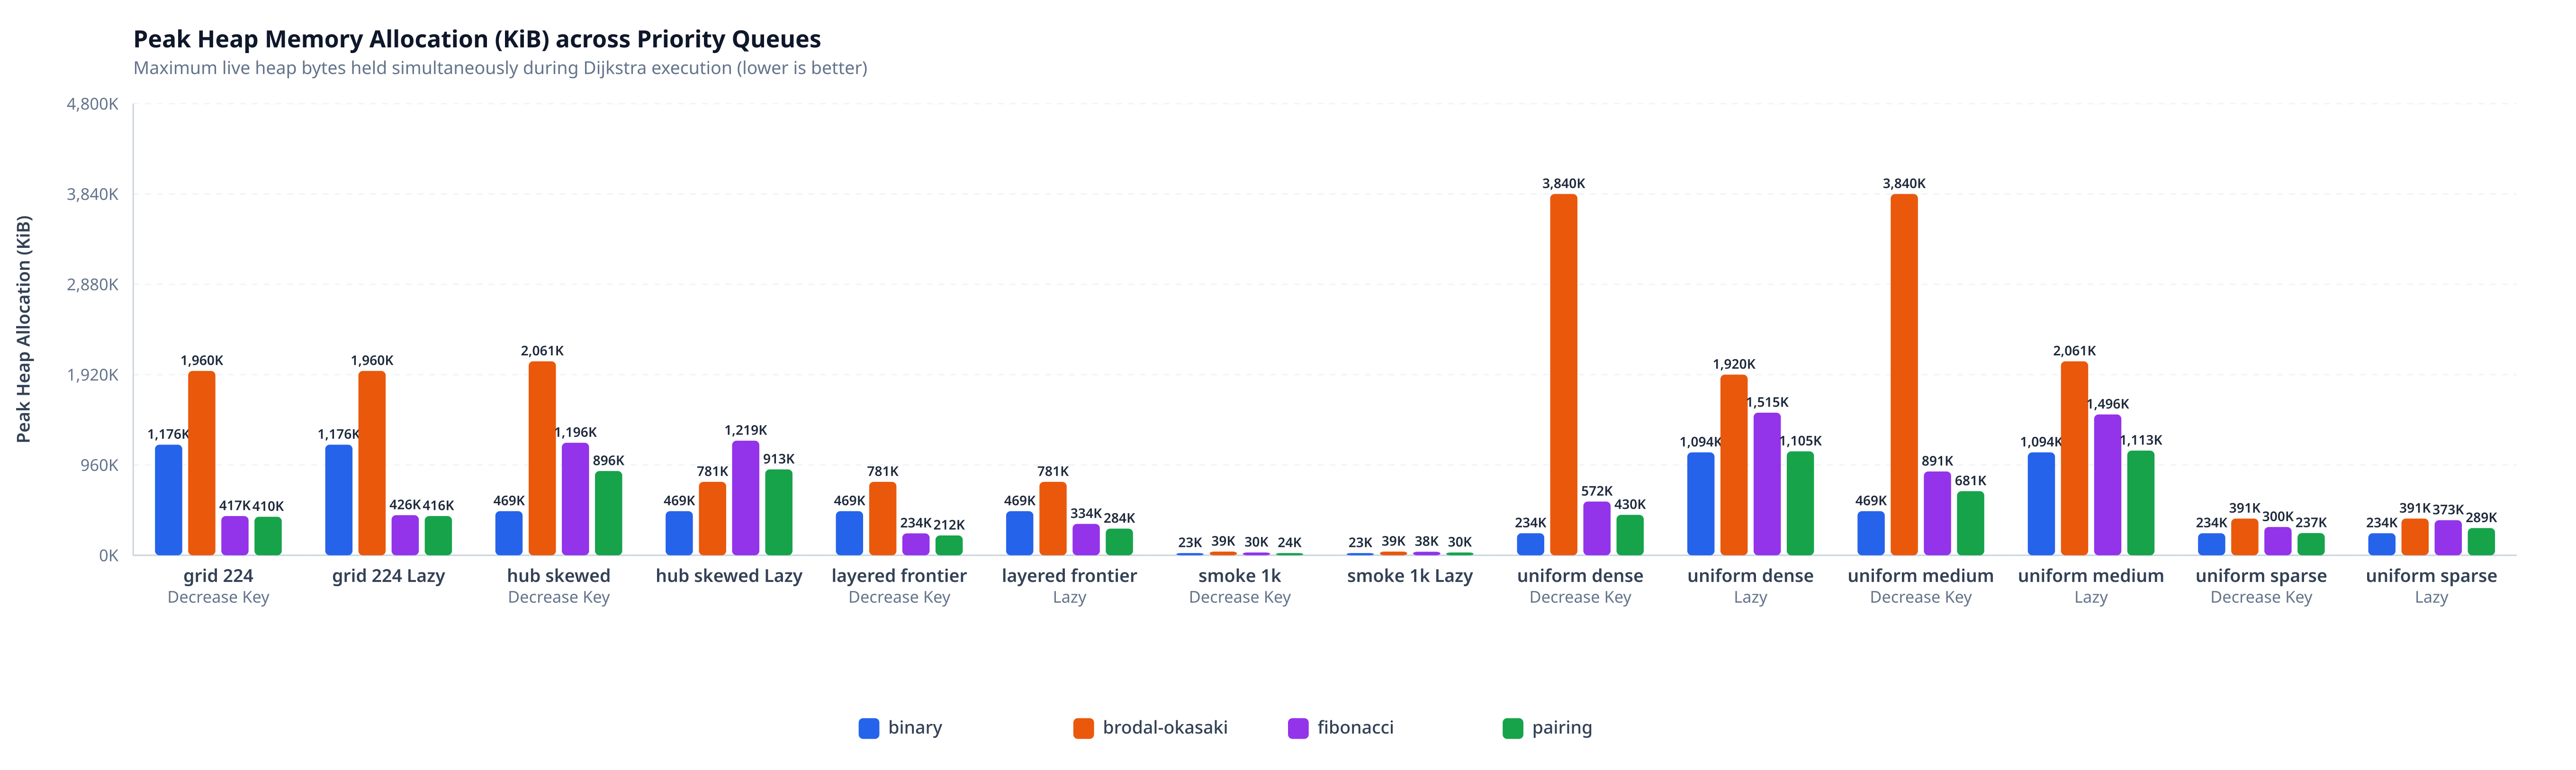
\includegraphics[width=0.95\textwidth]
    {frozen_results/figures/report_charts/mem/peak_heap_memory.png}
  \caption{Peak heap allocation across heap implementations, input graphs, and
  Dijkstra variants.}
  \label{fig:peak-heap-memory}
\end{figure}

\begin{figure}[H]
  \centering
  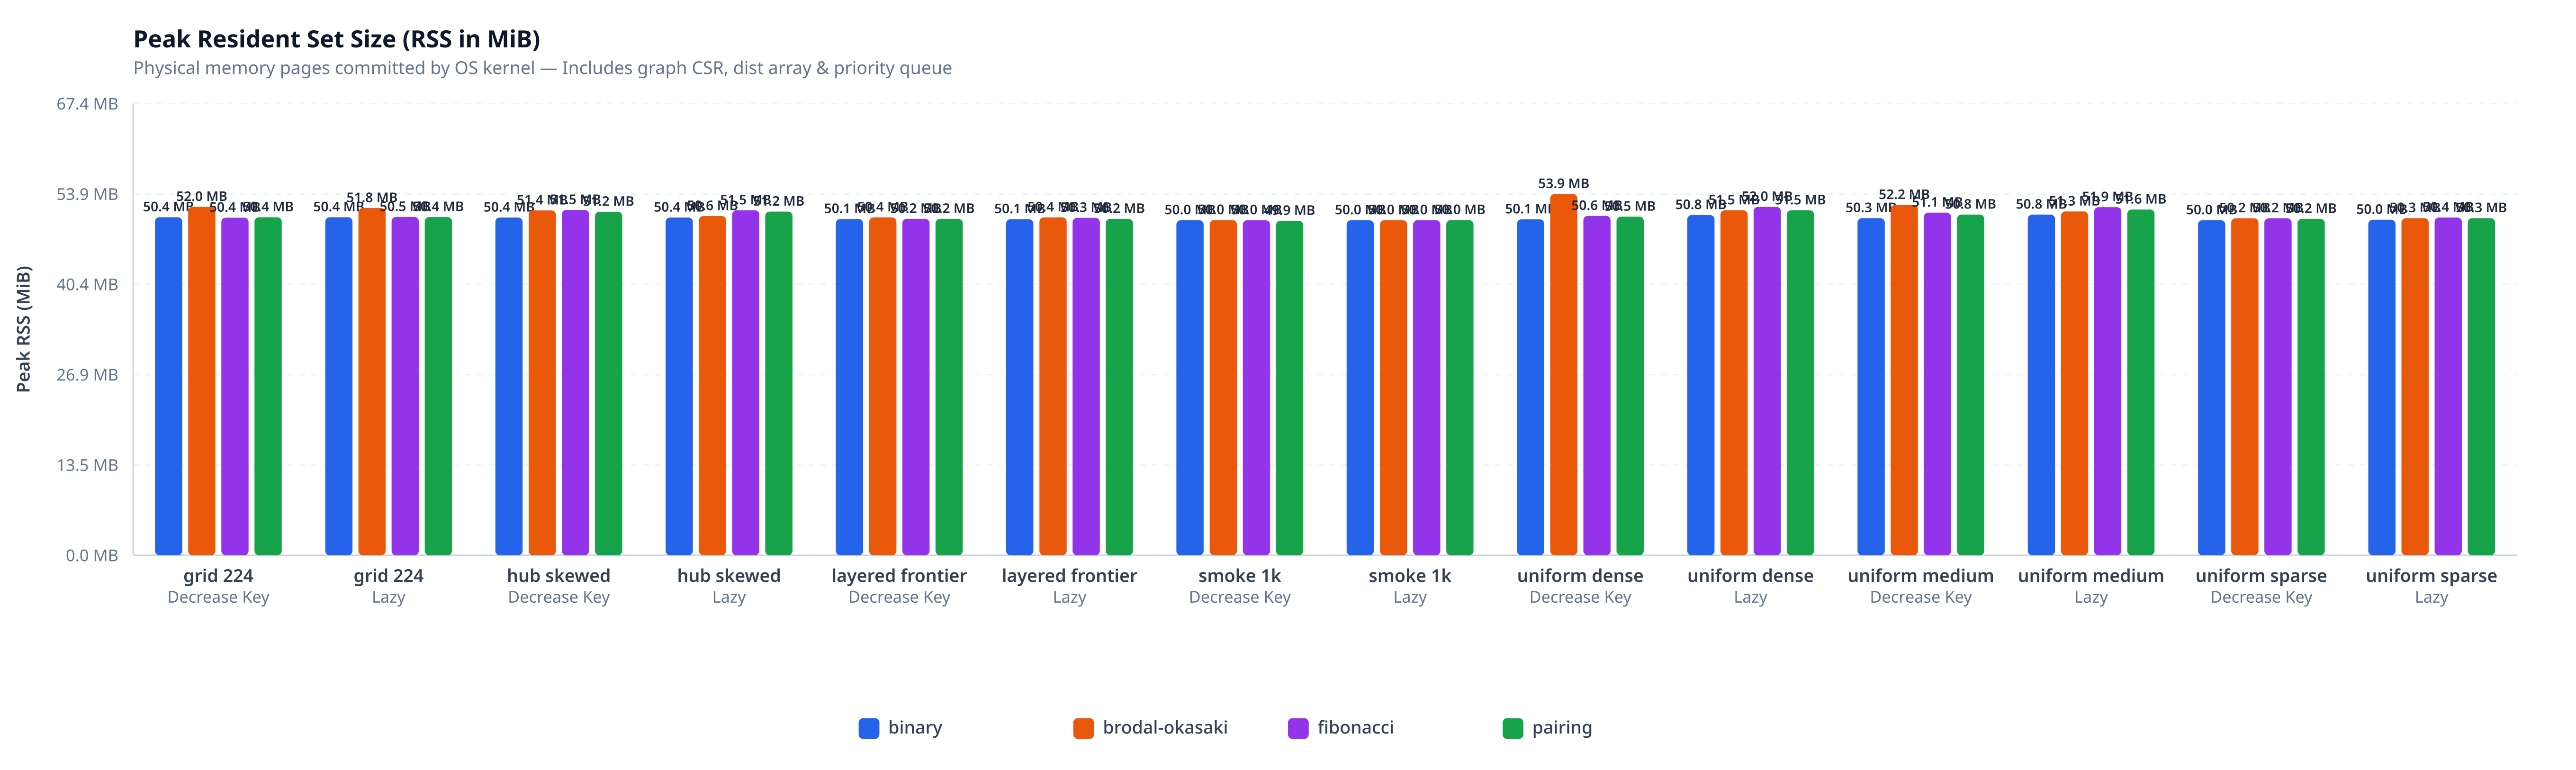
\includegraphics[width=0.95\textwidth]
    {frozen_results/figures/report_charts/mem/peak_rss_footprint.png}
  \caption{Peak resident set size across heap implementations, input graphs,
  and Dijkstra variants.}
  \label{fig:peak-rss-memory}
\end{figure}

The binary heap generally has the lowest peak heap allocation. Its contiguous
array representation stores queue entries compactly, with limited additional
metadata for position tracking. The pointer-based pairing and Fibonacci heaps
require per-node allocations and structural links, which increases their
memory footprint. The Brodal--Okasaki implementation also incurs additional
storage for its buffer and tree bookkeeping.

Peak memory increases as graph size and relaxation activity increase. The
effect is especially visible for the denser and layered inputs, where the
priority queue processes a larger active frontier. Lazy Dijkstra can further
increase memory usage because stale entries remain in the queue until they are
removed.

The resident set size follows the same broad pattern but includes memory
allocated outside the priority queue, including the graph representation and
runtime overhead. Consequently, differences in peak RSS are smaller than
differences in peak heap allocation for some inputs. No negative allocation
values or leaks were recorded in the frozen results.

\subsubsection{Allocator Activity}

Figure~\ref{fig:allocator-pressure} shows allocator activity across the heap
implementations and input graphs.

\begin{figure}[H]
  \centering
  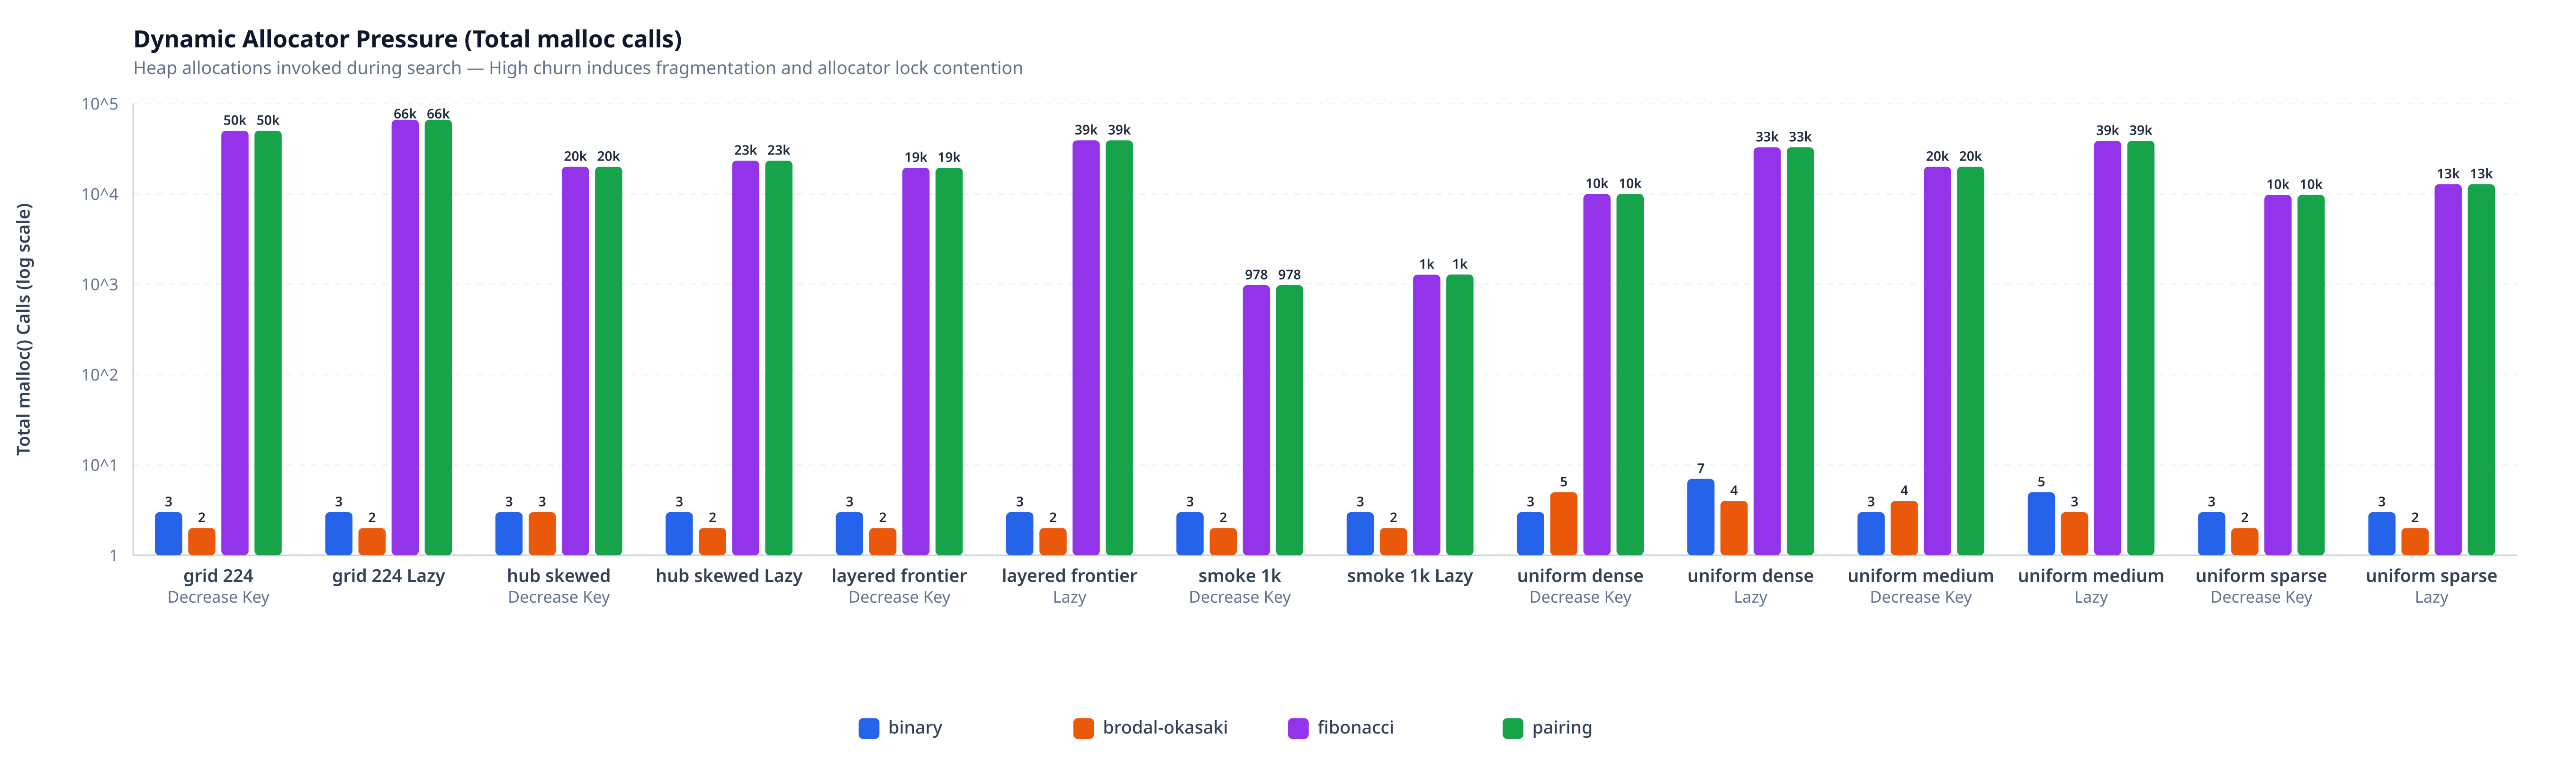
\includegraphics[width=0.95\textwidth]
    {frozen_results/figures/report_charts/mem/allocator_pressure.png}
  \caption{Dynamic allocation activity across heap implementations, input
  graphs, and Dijkstra variants.}
  \label{fig:allocator-pressure}
\end{figure}

The binary and Brodal--Okasaki implementations perform very few allocation
operations because they primarily use preallocated or buffer-based storage.
In contrast, the pairing and Fibonacci heaps allocate individual nodes, which
results in substantially more \code{malloc} and \code{free} calls.

Lazy processing generally increases allocator activity for the pointer-based
heaps because duplicate queue entries must be created and later released. The
increase is most visible on the medium, dense, and layered graphs, where more
relaxations produce more stale entries. All configurations report matching
allocation and free counts with zero leaked bytes, indicating that the
additional allocation activity is temporary rather than caused by unreleased
memory.

These results support the runtime and peak-memory measurements: allocation
frequency and allocator overhead contribute to the higher cost of the
pointer-based implementations, particularly when lazy Dijkstra increases the
number of queue entries.

\subsection{Cross-Experiment Analysis}

Taken together, the runtime, hardware-counter, and memory results consistently
favour the binary heap. Its contiguous array representation gives it the
lowest runtime in every tested configuration, while also limiting allocation
activity and peak heap usage. The pairing heap is generally the second-fastest,
but its pointer-based structure introduces additional memory and allocation
overhead.

The Fibonacci and Brodal--Okasaki heaps do not overcome their higher constant
costs in this workload, despite their stronger theoretical bounds for selected
priority-queue operations. The hardware measurements support this result:
the slower implementations retire more instructions and incur more cache
misses per vertex, and Brodal-Okasaki additionally loses efficiency to branch
mispredictions.

The choice of Dijkstra variant also matters. Decrease-key is faster for the
binary, pairing, and Fibonacci heaps because it avoids stale queue entries.
The Brodal--Okasaki implementation benefits from lazy processing because its
decrease-key operation is comparatively expensive. Overall, graph structure
and heap implementation interact substantially, so theoretical complexity
alone does not predict the observed end-to-end performance.